\documentclass{article}
\usepackage[utf8]{inputenc}

\usepackage{amsmath}
\usepackage{amssymb}
\usepackage{arydshln}

\usepackage{tikz}
\usetikzlibrary{positioning,arrows,decorations.markings}

\newcommand{\tjzm}{$t$-$J^z$~model}
\newcommand{\ket}[1]{\left\vert #1 \right\rangle}
\newcommand{\bra}[1]{\left\langle #1 \right\vert}
\newcommand{\abs}[1]{\left\vert #1 \right\vert}

\def\K{%
    \operatornamewithlimits{%
        \mathchoice{% * Display style
            \vcenter{\hbox{\huge $\mathcal{K}$}}%
        }{%           * Text style
            \vcenter{\hbox{\Large $\mathcal{K}$}}%
        }{%           * Script style
            \mathrm{\mathcal{K}}%
        }{%           * Script script style
            \mathrm{\mathcal{K}}%
        }
    }
}

\def\composition{\operatornamewithlimits{\circ}}

\title{Rotational ARPES for 2D t-Jz model: Self-avoiding walks approximation}
\author{piotr.wrzosek@fuw.edu.pl}
\date{July 2021}

\begin{document}

\maketitle

\section{Rotational Greens Function}
Rotational degrees of freedom can be introduced by substituting standard electron annihilation $\tilde{c}_j$ in the definition of the local Greens function by
\begin{equation}
    R_{\sigma, m}(j) = \frac{1}{2}\sum_{i:\langle i,j \rangle} e^{i m \varphi_{i-j}} \sum_{\sigma'} \tilde{c}_{j,\sigma'}^{\dag} \tilde{c}_{i,\sigma'} \tilde{c}_{j,\sigma},
\end{equation}
where $\varphi_{i-j}$ is equal to the angle (in radians) between $x$ axis and the bond between sites j and i (starting at j and ending at i) and the sum over $i:\langle i,j \rangle$ means sum over all sites $i$ that are nearest neighbors of site $j$. Moreover, phases are multiplied by the parameter $m \in \{0,1,2,3\}$.
The above states that the hole is created at site $j$ and is being propagated to nearest neighboring sites with phase factors corresponding to the direction in which the hole moves.

The above may be generalized to include multiple moves of the hole. For $n$ moves we could write,
\begin{equation}
\begin{split}
    R_{\sigma, m_1, m_2, ..., m_n}(j_0) = \frac{1}{2^n}\left(
    \sum_{j_1:\langle j_1,j_0 \rangle} 
    \sum_{j_2:\langle j_2,j_1 \rangle} 
    \hdots
    \sum_{j_n:\langle j_n,j_{n-1} \rangle}
        \right)
    e^{i \sum_{l = 1}^n m_l \varphi_{j_l-j_{l-1}}} 
    \times \\ \times 
    \sum_{\sigma_1, \sigma_2, ..., \sigma_n}
    \tilde{c}_{j_{n-1},\sigma_n}^{\dag} \tilde{c}_{j_n,\sigma_n}
    \hdots
    \tilde{c}_{j_1,\sigma_2}^{\dag} \tilde{c}_{j_2,\sigma_2}
    \tilde{c}_{j_0,\sigma_1}^{\dag} \tilde{c}_{j_1,\sigma_1} \tilde{c}_{j_0,\sigma},
\end{split}
\end{equation}
where $m_i \in \{0,1,2,3\}$.
Our goal is to calculate (or to find a convenient algorithm for calculating) the above quantity in the following scenarios:
\begin{enumerate}
    \item any number $n$ of moves on the Bethe lattice,
    \item any number $n$ of moves for the self-avoiding walks approximation on the 2D square lattice.
\end{enumerate}

\section{Notation}
Before we start investigating the two cases mentioned in the previous section we need a notation that would allow us to make use of the symmetries of the system, both for the Bethe and the 2D square lattice case. Thus, let us start with introduction of definitions below:
\begin{enumerate}
    \item \textit{Lattice origin} (or simply \textit{origin}) - a particular site of the lattice chosen as the center of the lattice. For clarity, we set the origin to be located at position $\vec{r} = 0$ in any arbitrary coordinate system.
    
    \item \textit{Ground state} denoted as $\ket{0_\sigma}$ - state with one electron per site, where nearest neighboring electrons are anti-parallel; also called \textit{Ising} antiferromagnet (AF); note there are 2 possible Ising AF states denoted here by spin $\sigma$ at the origin.
    
    \item $E_{0}$ - energy of the ground state; note the energy of each ground state is the same.
    
    \item \textit{Initial state} denoted as $\ket{I_\sigma}$ - state that is obtained from the ground state by removing an electron from the origin, i.e. $c_{0,\sigma}\ket{0_\sigma}$. To shorten the notation we will often omit the index $\sigma$ and simply write $\ket{I}$.
    
    \item \textit{Coordination number} - denotes how many neighboring sites there is for each site in the lattice, e.g. for 2D square lattice $z = 4$.
    
    \item \textit{Move of the hole} - process of electron tunneling to the neighboring unoccupied site resulting in the motion of such unoccupied site in the opposite direction; mathematically expressed as $\sum_{\sigma} \tilde{c}_{j(i),\sigma}^{\dag} \tilde{c}_{i,\sigma}$, where $j(i)$ denotes site $j$ in the nearest neighborhood of site $i$.
    
    \item $E$, $N$, $W = E^{-1}$, $S = N^{-1}$ - possible moves of the hole in the lattice with coordination number $z = 4$. We get rid of ambiguities by aligning the lattice with respect to Cartesian coordinates. This way we can say: $E$ - move in $x$ direction (i.e. to the \textit{east}), $N$ - move in $y$ direction (\textit{north}), $W$ - move in $-x$ direction (\textit{west}), $S$ - move in $-y$ direction (\textit{south}). The process describing no motion is simply the identity, $I$. For subsequent moves we present multiplication table:
    
    \begin{center}
        \begin{tabular}{c | c c c c c }
            $\cdot$  
                     & $I$ & $E$  & $N$  & $W$  & $S$  \\ 
            \hline
            $I$      & $I$ & $E$  & $N$  & $W$  & $S$  \\
            $E$      & $E$ & $EE$ & $EN$ & $I$  & $ES$ \\
            $N$      & $N$ & $NE$ & $NN$ & $NW$ & $I$  \\
            $W$      & $W$ & $I$  & $WN$ & $WW$ & $WS$ \\
            $S$      & $S$ & $SE$ & $I$  & $SW$ & $SS$
        \end{tabular}        
    \end{center}
    
    \item $D = \{E, N, W, S\}$ - set of possible moves of the hole in the lattice with coordination number $z = 4$
    
    \item $\ket{xyz} = zyx\ket{I}$ - state obtained as a result of the hole motion according to jumps $x, y, z$, e.g. $\ket{ENN} = NNE\ket{I}$, i.e. state obtained by placing the hole at the origin and moving it once to the east and then twice to the north. This example generalizes to any number of moves.

    \item $\varphi_E = 0$, $\varphi_N = \frac{\pi}{2}$, $\varphi_W = \pi$, $\varphi_S = \frac{3\pi}{2}$.
    
\end{enumerate}

\section{Bethe Lattice}
Superlattice of the \tjzm{} Hamiltonian spanned on the Bethe lattice starting form initial state is acyclic three. Thus there cannot be any momentum dependence in this case.

\subsection{Local Greens function of a single hole}
It is easy to notice that such superlattice is also a Bethe lattice itself. In this superlattice any two nodes (i.e. states) that are distant by the same number of branches (i.e. hops of the hole) from the initial state, are equivalent - there is no process that could distinguish between them. From such a tree structure the following Greens function of the single hole can be immediately written,
\begin{equation}
    G(\omega)^{-1} = G_0(\omega)^{-1} - z\Sigma_0(\omega), 
\end{equation}
\begin{equation}
    t^2\Sigma_n(\omega)^{-1} = G_{n+1}(\omega)^{-1} - (z-1)\Sigma_{n+1}(\omega),
\end{equation}
where,
\begin{equation}
    G_{n}(\omega)^{-1} = \omega - \left(
        1 - \delta_{n} + z + \left( z-2 \right) n 
    \right)\frac{J}{2},
\end{equation}
and $z$ is a coordination number. In the case of $z=4$ explicit form of the local Greens function is as follows,
\begin{equation}
    G(\omega) = \frac{1}{
        \omega - 2J - \frac{4t^2}{
            \omega - \frac{7}{2}J - \frac{3t^2}{
                \omega - \frac{9}{2}J - \frac{3t^2}{
                    \omega - \frac{11}{2}J - \hdots
                }
            }
        }
    }.
\label{eq:BetheGF}
\end{equation}

\subsection{Local Greens function with rotations}
Let us now investigate rotational Greens function calculated on the Bethe lattice. For clarity, we will start with $n = 1$ case and later generalize it to higher $n$ values. We are interested in the following quantity,
\begin{equation}
    G^{\text{rot}}_{m}(\omega) = 
    \bra{0_\sigma}R^{\dag}_{\sigma,m}(0) 
        \hat{G}(\omega)
    R_{\sigma,m}(0) \ket{0_\sigma}.
\end{equation}
where $\hat{G}(\omega) = (\omega - H + E_0)^{-1}$, and $H$ stands for the \tjzm{} Hamiltonian. Within the introduced notation of the hole moves in lattice with coordinate number $z=4$, which is the case we investigate, we can write,
\begin{equation}
    R_{\sigma,m}(0) \ket{0_\sigma} = \frac{1}{2}\sum_{\xi \in D}
    e^{i m\varphi_\xi}\xi\ket{I} = \frac{1}{2}\left(\ket{E} + 
    e^{i m\frac{\pi}{2}}\ket{N} + e^{im\pi}\ket{W} + 
    e^{i m\frac{3\pi}{2}}\ket{S}\right).
\end{equation}
Therefore we can express our rotational Greens function in the following way,
\begin{equation}
    G^{\text{rot}}_{m}(\omega) = 
    \frac{1}{4}\sum_{\xi, \xi' \in D}
        e^{i m(\varphi_\xi - \varphi_{\xi'})}
        \bra{\xi'}\hat{G}(\omega)\ket{\xi}.
\end{equation}
Now we need to calculate $\bra{\xi'}\hat{G}(\omega)\ket{\xi}$. There are few approaches to this problem, especially in this specific case. We will follow not the easiest but more general one.

Let us denote $\hat{H}(\omega) = (\omega - H + E_0)$ such that $\hat{G}(\omega) = \hat{H}(\omega)^{-1}$. Then let define basis $\mathcal{B}$ of all possible states of the system that are reachable by any number of moves on the Bethe lattice starting form the initial state $\ket{I}$. In basis $\mathcal{B}$ we have the matrix $\mathcal{M}(\hat{G}(\omega))_\mathcal{B}^\mathcal{B}$ of the propagator $\hat{G}(\omega)$ with matrix elements,
\begin{equation}
    G_{\eta', \eta}(\omega) = \bra{\eta'}\hat{G}(\omega)\ket{\eta},
\end{equation}
where $\eta = \xi_1 \xi_2 \xi_3 \hdots$, $\eta' = \xi'_1 \xi'_2 \xi'_3 \hdots$ and each $\xi_i, \xi'_i \in D$. 

Fortunately, we do not need all the matrix elements of $\hat{G}(\omega)$, only few specific. Moreover, we can take advantage of the symmetries of the system, namely,
\begin{align}
    G_{E, E}(\omega) &= G_{\xi, \xi}(\omega),
        \quad \xi \in D, \\
    G_{N, E}(\omega) &= G_{\xi', \xi}(\omega),
        \quad \xi, \xi' \in D \land \xi \neq \xi'.
\end{align}
The above leads to
\begin{equation}
    G^{\text{rot}}_{m}(\omega) = G_{E, E}(\omega) + 
    (e^{i m\frac{\pi}{2}} + e^{i m\pi} + e^{i m\frac{3\pi}{2}}) 
        G_{N, E}(\omega),
\end{equation}
so we need to find only two matrix elements of the propagator $\hat{G}(\omega)$. 
In general we can find those elements with cofactor matrix method,
\begin{equation}
    \mathcal{M}(\hat{G}(\omega))_\mathcal{B}^\mathcal{B} = 
    \frac{C^{T}(\omega)}{\det \mathcal{M}(\hat{H}(\omega))_\mathcal{B}^\mathcal{B}},
\end{equation}
where matrix $C = [C_{i,j}]$, coefficients $C_{i,j} = (-1)^{i+j}M_{i,j}$ and $M_{i,j}$ is the $(i,j)$-minor of the matrix $\mathcal{M}(\hat{H}(\omega))_\mathcal{B}^\mathcal{B}$ with $i$-th row and $j$-th column removed.

In order to see how the cofactor matrix method works on the simplest example let us derive Eq.~\eqref{eq:BetheGF}, namely,
\begin{equation}
    G(\omega) = \bra{I}\hat{G}(\omega)\ket{I} = G_{I,I}(\omega) = \frac{C_{I,I}(\omega)}{\det \mathcal{M}(\hat{H}(\omega))_\mathcal{B}^\mathcal{B}}.
\end{equation}
We start by calculating,
\begin{equation}
\begin{split}
    &\det \mathcal{M}(\hat{H}(\omega))_\mathcal{B}^\mathcal{B} =
    \det H^{(0)}(\omega) = \\ 
    &\left\vert
    \begin{array}{c|c|c|c|c}
        \omega - 2J & 
            \begin{array}{ccc} t & 0 & \cdots \end{array} &
            \begin{array}{ccc} t & 0 & \cdots \end{array} &
            \begin{array}{ccc} t & 0 & \cdots \end{array} &
            \begin{array}{ccc} t & 0 & \cdots \end{array} \\
        \hline
        \begin{array}{c} t \\ 0 \\ \vdots \end{array} & 
            \begin{array}{c} H^{(1)}(\omega) \end{array} & 0 & 0 & 0 \\
        \hline
        \begin{array}{c} t \\ 0 \\ \vdots \end{array} & 
            0 & \begin{array}{c} H^{(1)}(\omega) \end{array} & 0 & 0 \\
        \hline
        \begin{array}{c} t \\ 0 \\ \vdots \end{array} & 
            0 & 0 &\begin{array}{c} H^{(1)}(\omega) \end{array} & 0 \\
        \hline
        \begin{array}{c} t \\ 0 \\ \vdots \end{array} & 
            0 & 0 & 0 & \begin{array}{c} H^{(1)}(\omega) \end{array}
    \end{array}
    \right\vert.
\end{split}
\end{equation}
We notice that if matrix $H^{(1)}(\omega)$ was in lower triangular form we easily could bring matrix $H^{(0)}$ to lower triangular form too. This way the determinant would equal to the product of the diagonal elements of $H^{(0)}$. We also have,
\begin{equation}
    H^{(1)}(\omega) =  
    \left[
    \begin{array}{c|c|c|c}
        \omega - \frac{7}{2}J & 
            \begin{array}{ccc} t & 0 & \cdots \end{array} &
            \begin{array}{ccc} t & 0 & \cdots \end{array} &
            \begin{array}{ccc} t & 0 & \cdots \end{array} \\
        \hline
        \begin{array}{c} t \\ 0 \\ \vdots \end{array} & 
            \begin{array}{c} H^{(2)}(\omega) \end{array} & 0 & 0 \\
        \hline
        \begin{array}{c} t \\ 0 \\ \vdots \end{array} & 
            0 & \begin{array}{c} H^{(2)}(\omega) \end{array} & 0  \\
        \hline
        \begin{array}{c} t \\ 0 \\ \vdots \end{array} & 
            0 & 0 &\begin{array}{c} H^{(2)}(\omega) \end{array}
    \end{array}
    \right],
\end{equation}
so again if $H^{(2)}(\omega)$ is lower triangular, we can transform $H^{(1)}(\omega)$ to lower triangular form with ease. Such pattern repeats for any self-avoiding walk of the hole. This is not a restriction in our case, because walks on the Bethe lattice are always self-avoiding. By restricting ourselves to moves with $n$ jumps of the hole we notice the sequence ends with $H^{(n)}$ that indeed is in lower triangular form, as it is $1 \times 1$ matrix. Reducing matrices to lower triangular form sequentially by applying transformations that do not change the determinant and in the end taking the limit of $n\to\infty$,  we finally obtain,
\begin{equation}
\begin{split}
    &\det H^{(0)}(\omega) = \\ 
    &\left\vert
    \begin{array}{c|c|c|c|c}
        \omega - 2J - \frac{4t^2}{
            \omega - \frac{7}{2}J - \frac{3t^2}{
                \omega - \frac{9}{2}J - \frac{3t^2}{
                    \omega - \frac{11}{2}J - \hdots
                }
            }
        } & 
            0 & 0 & 0 & 0 \\
        \hline
        \begin{array}{c} t \\ 0 \\ \vdots \end{array} & 
            \begin{array}{c} T^{(1)}(\omega) \end{array} & 0 & 0 & 0 \\
        \hline
        \begin{array}{c} t \\ 0 \\ \vdots \end{array} & 
            0 & \begin{array}{c} T^{(1)}(\omega) \end{array} & 0 & 0 \\
        \hline
        \begin{array}{c} t \\ 0 \\ \vdots \end{array} & 
            0 & 0 &\begin{array}{c} T^{(1)}(\omega) \end{array} & 0 \\
        \hline
        \begin{array}{c} t \\ 0 \\ \vdots \end{array} & 
            0 & 0 & 0 & \begin{array}{c} T^{(1)}(\omega) \end{array}
    \end{array}
    \right\vert,
\end{split}
\end{equation}
and for $k > 0$,
\begin{equation}
    T^{(k)}(\omega) =  
    \left[
    \begin{array}{c|c|c|c}
        \omega - \frac{5+2k}{2}J - \frac{3t^2}{
            \omega - \frac{7+2k}{2}J - \hdots
        } & 
            0 & 0 & 0 \\
        \hline
        \begin{array}{c} t \\ 0 \\ \vdots \end{array} & 
            \begin{array}{c} T^{(k+1)}(\omega) \end{array} & 0 & 0 \\
        \hline
        \begin{array}{c} t \\ 0 \\ \vdots \end{array} & 
            0 & \begin{array}{c} T^{(k+1)}(\omega) \end{array} & 0  \\
        \hline
        \begin{array}{c} t \\ 0 \\ \vdots \end{array} & 
            0 & 0 &\begin{array}{c} T^{(k+1)}(\omega) \end{array}
    \end{array}
    \right],
\end{equation}
where $T^{(k)}(\omega)$ corresponds to $H^{(k)}(\omega)$ after triangulation. 
Now we can write down the determinant,
\begin{equation}
    \det \mathcal{M}(\hat{H}(\omega))_\mathcal{B}^\mathcal{B} = 
    \left(\omega - 2J - \frac{4t^2}{
            \omega - \frac{7}{2}J - \frac{3t^2}{
                \omega - \frac{9}{2}J - \frac{3t^2}{
                    \omega - \frac{11}{2}J - \hdots
                }
            }
        }\right) 
        \left(\det T^{(1)}(\omega) \right)^4,
\end{equation}
where for $k > 0$,
\begin{equation}
    \det T^{(k)}(\omega) = 
        \left(\omega - \frac{5+2k}{2}J - \frac{3t^2}{
            \omega - \frac{7+2k}{2}J - \hdots
        }\right) 
        \left(\det T^{(k+1)}(\omega) \right)^3.
        \label{eq:det_triangular_recursive}
\end{equation}
The last part is to calculate $C_{I,I}$ which is the determinant of the $\mathcal{M}(\hat{H}(\omega))_\mathcal{B}^\mathcal{B}$ with first row and first column removed. Luckily, we already have it calculated,
\begin{equation}
    C_{I,I}(\omega) = \left(\det T^{(1)}(\omega) \right)^4.
\end{equation}
This way we obtain,
\begin{equation}
    G(\omega) = G_{I,I}(\omega) = \frac{C_{I,I}(\omega)}{\det \mathcal{M}(\hat{H}(\omega))_\mathcal{B}^\mathcal{B}} = \frac{1}{
        \omega - 2J - \frac{4t^2}{
            \omega - \frac{7}{2}J - \frac{3t^2}{
                \omega - \frac{9}{2}J - \frac{3t^2}{
                    \omega - \frac{11}{2}J - \hdots
                }
            }
        }
    },
\end{equation}
which is exactly the same as in the Eq.~\eqref{eq:BetheGF}. 

Now, let go back to the investigated rotational Greens function with $n=1$. By taking advantage of the system symmetries, we determined that it is enough to calculate $G_{E, E}(\omega)$ and $G_{N, E}(\omega)$. Since we already know $\det \mathcal{M}(\hat{H}(\omega))_\mathcal{B}^\mathcal{B}$, it is enough for us to calculate corresponding cofactors, namely $C_{E,E}(\omega)$ and $C_{E, N}(\omega)$. We start with the diagonal one,
\begin{equation}
\begin{split}
    &C_{E,E}(\omega) = (-1)^2 \times \\ 
    &\left\vert
    \begin{array}{c|c|c|c|c}
        \omega - 2J & 0 &
            \begin{array}{ccc} t & 0 & \cdots \end{array} &
            \begin{array}{ccc} t & 0 & \cdots \end{array} &
            \begin{array}{ccc} t & 0 & \cdots \end{array} \\
        \hline
        0 & 
            \begin{array}{c;{2pt/2pt}c;{2pt/2pt}c}
                H^{(2)}(\omega) & 0 & 0 \\
                \hdashline[2pt/2pt]
                0 & H^{(2)}(\omega) & 0  \\
                \hdashline[2pt/2pt]
                0 & 0 & H^{(2)}(\omega)
            \end{array} & 0 & 0 & 0 \\
        \hline
        \begin{array}{c} t \\ 0 \\ \vdots \end{array} & 
            0 & H^{(2)}(\omega) & 0 & 0 \\
        \hline
        \begin{array}{c} t \\ 0 \\ \vdots \end{array} & 
            0 & 0 & H^{(2)}(\omega) & 0 \\
        \hline
        \begin{array}{c} t \\ 0 \\ \vdots \end{array} & 
            0 & 0 & 0 & H^{(2)}(\omega)
    \end{array}
    \right\vert,
\end{split}
\end{equation}
and immediately notice that,
\begin{equation}
\begin{split}
    &C_{E,E}(\omega) = \\ 
    &\left\vert
    \begin{array}{c|c|c|c}
        \omega - 2J &
            \begin{array}{ccc} t & 0 & \cdots \end{array} &
            \begin{array}{ccc} t & 0 & \cdots \end{array} &
            \begin{array}{ccc} t & 0 & \cdots \end{array} \\
        \hline
        \begin{array}{c} t \\ 0 \\ \vdots \end{array} & 
            H^{(2)}(\omega) & 0 & 0 \\
        \hline
        \begin{array}{c} t \\ 0 \\ \vdots \end{array} & 
            0 & H^{(2)}(\omega) & 0 \\
        \hline
        \begin{array}{c} t \\ 0 \\ \vdots \end{array} & 
            0 & 0 & H^{(2)}(\omega)
    \end{array}
    \right\vert 
    \times \left(\det H^{(2)}(\omega)\right)^3 \\
    =  &\left(\omega - 2J - \frac{3t^2}{
            \omega - \frac{7}{2}J - \frac{3t^2}{
                \omega - \frac{9}{2}J - \frac{3t^2}{
                    \omega - \frac{11}{2}J - \hdots
                }
            }
        }\right) 
    \left(\det T^{(1)}(\omega) \right)^3 \left(\det T^{(2)}(\omega)\right)^3 \\
    =  &\frac{
            \omega - 2J - \frac{3t^2}{
                \omega - \frac{7}{2}J - \frac{3t^2}{
                    \omega - \frac{9}{2}J - \frac{3t^2}{
                        \omega - \frac{11}{2}J - \hdots
                    }
                }
            }
        }{
            \omega - \frac{7}{2}J - \frac{3t^2}{
                \omega - \frac{9}{2}J - \frac{3t^2}{
                    \omega - \frac{11}{2}J - \hdots
                }
            }        
        }
    \left(\det T^{(1)}(\omega) \right)^4 \\
    =  &\frac{1}{t^2}
        \Sigma_0(\omega)\left(G(\omega)^{-1} + \Sigma_0(\omega)\right) 
        \left(\det T^{(1)}(\omega) \right)^4.
\end{split}
\end{equation}    
Thus we obtain,
\begin{equation}
    G_{E,E}(\omega) = \frac{C_{E,E}(\omega)}{\det \mathcal{M}(\hat{H}(\omega))_\mathcal{B}^\mathcal{B}} = 
    \frac{1}{t^2}\left(\Sigma_0(\omega) + \Sigma_0(\omega)G(\omega)\Sigma_0(\omega)\right).
\end{equation}
And finally for the off-diagonal coefficient $C_{E,N}(\omega)$ we remove the row corresponding to the position of the state $\ket{E}$ and the column corresponding to the state $\ket{N}$, so we have,
\begin{equation}
\begin{split}
    &C_{E,N}(\omega) = (-1)^{4 + \dim H^{(1)}(\omega)} \times \\ 
    &\left\vert
    \begin{array}{c|c|c|c|c}
        \omega - 2J & 
            \begin{array}{cccc} t & 0 & \cdots & 0 \end{array} & 
            0 &
            \begin{array}{ccc} t & 0 & \cdots \end{array} &
            \begin{array}{ccc} t & 0 & \cdots \end{array} \\
        \hline
        0 & B^{(1)}_{1,0}(\omega) & 0 & 0 & 0 \\
        \hline
        \begin{array}{c} t \\ 0 \\ \vdots \\ 0 \end{array} & 
            0 & B^{(1)}_{0,1}(\omega) & 0 & 0 \\
        \hline
        \begin{array}{c} t \\ 0 \\ \vdots \end{array} & 
            0 & 0 &\begin{array}{c} H^{(1)}(\omega) \end{array} & 0 \\
        \hline
        \begin{array}{c} t \\ 0 \\ \vdots \end{array} & 
            0 & 0 & 0 & \begin{array}{c} H^{(1)}(\omega) \end{array}
    \end{array}
    \right\vert,
\end{split}
\end{equation}
where we define $\dim A = n$ for $A\in\mathcal{M}_{n \times n}$ and
\begin{equation}
    B^{(1)}_{1,0}(\omega) = \left[
        \begin{array}{c;{2pt/2pt}c;{2pt/2pt}c;{2pt/2pt}c}
                \begin{array}{c} t \\ 0 \\ \vdots \end{array} 
                & H^{(2)}(\omega) & 0 & 0 \\
                \hdashline[2pt/2pt]
                \begin{array}{c} t \\ 0 \\ \vdots \end{array}
                & 0 & H^{(2)}(\omega) & 0  \\
                \hdashline[2pt/2pt]
                \begin{array}{c} t \\ 0 \\ \vdots \end{array}
                & 0 & 0 & H^{(2)}(\omega)
    \end{array} \right].
\end{equation}
Here $B^{(1)}_{0,1}(\omega) = B^{(1)}_{1,0}(\omega)^\dag$ is $H^{(1)}(\omega)$ with first column removed. We start by transforming $H^{(1)}(\omega)$ to lower triangular form $T^{(1)}(\omega)$ and reducing transition coefficients in the first row of the upper part of the matrix located above entries of $T^{(1)}(\omega)$,
\begin{equation}
\begin{split}
    &C_{E,N}(\omega) = (-1)^{4 + \dim H^{(1)}(\omega)} \times\\ 
    &\left\vert
    \begin{array}{c|c|c|c|c}
        G_0(\omega)^{-1} - 2\Sigma_0(\omega) & 
            \begin{array}{cccc} t & 0 & \cdots & 0 \end{array} & 
            0 & 0 & 0 \\
        \hline
        0 & B^{(1)}_{1,0}(\omega) & 0 & 0 & 0 \\
        \hline
        \begin{array}{c} t \\ 0 \\ \vdots \\ 0 \end{array} & 
            0 & B^{(1)}_{0,1}(\omega) & 0 & 0 \\
        \hline
        \begin{array}{c} t \\ 0 \\ \vdots \end{array} & 
            0 & 0 &\begin{array}{c} T^{(1)}(\omega) \end{array} & 0 \\
        \hline
        \begin{array}{c} t \\ 0 \\ \vdots \end{array} & 
            0 & 0 & 0 & \begin{array}{c} T^{(1)}(\omega) \end{array}
    \end{array}
    \right\vert.
\end{split}
\end{equation}
Then, we triangulate matrices $H^{(2)}(\omega)$ in $B^{(1)}_{0,1}(\omega)$. This allows us to reduce all the entries in the first row of matrix $B^{(1)}_{0,1}(\omega)$ to 0. This way the row with index $1 + \dim H^{(1)}(\omega)$ in the matrix, whose determinant is being calculated, is zero everywhere but in the first column. Thus we can use it to reduce the first column of the matrix.
\begin{equation}
\begin{split}
    &C_{E,N}(\omega) = (-1)^{\dim H^{(1)}(\omega)} \times\\ 
    &\left\vert
    \begin{array}{c|c|c|c|c}
        0 & 
            \begin{array}{cccc} t & 0 & \cdots & 0 \end{array} & 
            0 & 0 & 0 \\
        \hline
        0 & B^{(1)}_{1,0}(\omega) & 0 & 0 & 0 \\
        \hline
        \begin{array}{c} t \\ 0 \\ \vdots \\ 0 \end{array} & 
            0 & 
            \begin{array}{c;{2pt/2pt}c;{2pt/2pt}c}
                0 & 0 & 0 \\
                \hdashline[2pt/2pt]
                T^{(2)}(\omega) & 0 & 0 \\
                \hdashline[2pt/2pt]
                0 & T^{(2)}(\omega) & 0  \\
                \hdashline[2pt/2pt]
                0 & 0 & T^{(2)}(\omega)
            \end{array}            
            & 0 & 0 \\
        \hline
        \begin{array}{c} 0 \\ 0 \\ \vdots \end{array} & 
            0 & 0 &\begin{array}{c} T^{(1)}(\omega) \end{array} & 0 \\
        \hline
        \begin{array}{c} 0 \\ 0 \\ \vdots \end{array} & 
            0 & 0 & 0 & \begin{array}{c} T^{(1)}(\omega) \end{array}
    \end{array}
    \right\vert.
\end{split}
\end{equation}
We see the first row has the only non-zero element in the second column. We use it to reduce all the other coefficients in this column, i.e. coefficients in the first column of matrix $B^{(1)}_{1,0}(\omega)$. Then we push row $1 + \dim H^{(1)}(\omega)$ up to the top swapping it with consecutive rows what introduce sign $(-1)^{1 + 3\dim H^{(2)}(\omega)}$ change in determinant,
\begin{equation}
\begin{split}
    &C_{E,N}(\omega) = (-1)^{\dim H^{(1)}(\omega)} (-1)^{1 + 3\dim H^{(2)}(\omega)} \times\\ 
    &\left\vert
    \begin{array}{c|c|c|c|c}
        t & 0 & 0 & 0 & 0 \\
        \hline
        0 & 
        \begin{array}{c;{2pt/2pt}c;{2pt/2pt}c;{2pt/2pt}c}
            t & 0 & 0 & 0 \\
            \hdashline[2pt/2pt]
            0 & T^{(2)} & 0 & 0 \\
            \hdashline[2pt/2pt]
            0 & 0 & T^{(2)} & 0 \\
            \hdashline[2pt/2pt]
            0 & 0 & 0 & T^{(2)} \\
        \end{array}        
        & 0 & 0 & 0 \\
        \hline
        0 & 
            0 & 
            \begin{array}{c;{2pt/2pt}c;{2pt/2pt}c}
                T^{(2)} & 0 & 0 \\
                \hdashline[2pt/2pt]
                0 & T^{(2)} & 0  \\
                \hdashline[2pt/2pt]
                0 & 0 & T^{(2)}
            \end{array}            
            & 0 & 0 \\
        \hline
        0 & 
            0 & 0 &\begin{array}{c} T^{(1)} \end{array} & 0 \\
        \hline
        0 & 
            0 & 0 & 0 & \begin{array}{c} T^{(1)} \end{array}
    \end{array}
    \right\vert,
\end{split}
\end{equation}
where $T^{(2)} = T^{(2)}(\omega)$. We see that obtained matrix is lower triangular and we notice,
\begin{equation}
    (-1)^{\dim H^{(1)}(\omega)} (-1)^{1 + 3\dim H^{(2)}(\omega)} =
    (-1)^{2\dim H^{(1)}(\omega)} = 1,
\end{equation}
thus we have,
\begin{equation}
    C_{E,N}(\omega) = t^2 
        \left(\det T^{(1)}(\omega) \right)^2 
        \left(\det T^{(2)}(\omega) \right)^6 
    =   \frac{1}{t^2} 
        \Sigma_0(\omega)^2 
        \left(\det T^{(1)}(\omega) \right)^4.
\end{equation}
This way we finally obtain,
\begin{equation}
    G_{N,E} = \frac{C_{E,N}}
        {\det \mathcal{M}(\hat{H}(\omega))_\mathcal{B}^\mathcal{B}} =
    \frac{1}{t^2} 
        \Sigma_0(\omega)G(\omega)\Sigma_0(\omega).
\end{equation}
In the end, we obtain the following form of the rotational Greens function,
\begin{equation}
    G^{\text{rot}}_{m}(\omega) = \frac{1}{t^2}
        \Sigma_0(\omega) + 
        \frac{4\delta_{m}}{t^2}
        \Sigma_0(\omega)G(\omega)\Sigma_0(\omega),
\end{equation}
where
\begin{equation}
    \delta_{m} = \frac{1}{4} \sum_{k=0}^{3} e^{i \frac{k\pi}{2} m}.
\end{equation}

\subsection{General form of the cofactor}
We could see how to find rotational Greens function for a single hole move. Now let investigate general case of hole moving $n$ times from the origin. In this case, we look for the coefficients of the Greens function in the basis $\mathcal{B}$, 
\begin{equation}
    G_{\eta', \eta}(\omega) = \bra{\eta'}\hat{G}(\omega)\ket{\eta},
\end{equation}
where $\eta = \xi_1 \xi_2 \xi_3 \hdots$, $\eta' = \xi'_1 \xi'_2 \xi'_3 \hdots$ and each $\xi_i, \xi'_i \in D$. Before we move forward let us introduce the following notation,
\begin{equation}
    \Gamma_k^{(s)}(\omega) = G_{k}(\omega)^{-1} - s\Sigma_{k}(\omega),
\end{equation}
such that 
\begin{equation}
    \Gamma_0^{(4)}(\omega) = G(\omega)^{-1}
\end{equation}
and for $k > 0$ we have,
\begin{equation}
    \det T^{(k)}(\omega) = 
        \Gamma_k^{(3)}(\omega) 
        \left(\det T^{(k+1)}(\omega) \right)^3.
        \label{eq:det_recursive_gamma}
\end{equation}


Our goal is to find the cofactor $C_{\eta, \eta'}$, which is equal to the determinant of the matrix of the operator $\omega - H + E_0$ in basis $\mathcal{B}$ with row corresponding to state $\eta$ and column corresponding to state $\eta'$ removed, multiplied by $(-1)^{i+j}$ where $i,j$ denote indices of the removed row and column.

After removing $i$-th row and $j$-th column the matrix is in \textit{imbalanced} form, i.e. some previously diagonal elements may be now shifted from the diagonal. We can take row and a column with opposite indices, i.e. $j$ for the row and $i$ for the column (where we refer to the indices of a matrix before removing any rows/columns) and balance the matrix out by moving both the row and the column to the first row and first column respectively. This will bring previously diagonal elements back to the diagonal. When calculating determinant this will result in additional factor of $(-1)^{i+j-1}$ for swapping rows/columns. Together with the coefficient from the definition of the cofactor we simply get $(-1)^{2i+2j-1} = -1$, which means we do not need to know position of states $\eta, \eta'$ in the basis at all, provided that we use the described scheme to balance out the matrix. To paint a picture, we present below the calculated previously cofactor $C_{E,N}$ with the described scheme of balancing its matrix applied,
\begin{equation}
\begin{split}
    &C_{E,N}(\omega) = (-1) \times\\ 
    &\left\vert
    \begin{array}{c|c|c|c|c|c}
        0 & t & 0 & B^T & 0 & 0 \\
        \hline
        t & G_0^{-1} & 0 & 0 
            & t~~0~~\cdots        
            & t~~0~~\cdots
        \\
        \hline
        B & 0 &
        \begin{array}{c;{2pt/2pt}c;{2pt/2pt}c}
            H^{(2)} & 0 & 0 \\
            \hdashline[2pt/2pt]
            0 & H^{(2)} & 0 \\
            \hdashline[2pt/2pt]
            0 & 0 & H^{(2)} \\
        \end{array}        
        & 0 & 0 & 0 \\
        \hline
        0 & 0 & 0 &
            \begin{array}{c;{2pt/2pt}c;{2pt/2pt}c}
                H^{(2)} & 0 & 0 \\
                \hdashline[2pt/2pt]
                0 & H^{(2)} & 0  \\
                \hdashline[2pt/2pt]
                0 & 0 & H^{(2)}
            \end{array}            
        & 0 & 0 \\
        \hline
        0 & \begin{array}{c}
             t \\ 0 \\ \vdots
        \end{array} &
            0 & 0 &\begin{array}{c} H^{(1)} \end{array} & 0 \\
        \hline
        0 & \begin{array}{c}
             t \\ 0 \\ \vdots
        \end{array} &
            0 & 0 & 0 & \begin{array}{c} H^{(1)} \end{array}
    \end{array}
    \right\vert,
\end{split}
\end{equation}
where
\begin{equation}
    B^T = \left[\begin{array}{c;{2pt/2pt}c;{2pt/2pt}c} 
        \begin{array}{cccc}
             t & 0 & \cdots & 0
        \end{array} &
        \begin{array}{cccc}
             t & 0 & \cdots & 0
        \end{array} &
        \begin{array}{cccc}
             t & 0 & \cdots & 0
        \end{array} 
    \end{array}\right].
\end{equation}

We can notice that in the stated above matrix there is a block column with zeros everywhere besides the diagonal block. Such column appears since we removed a single row that was placed right above the mentioned diagonal block. Analogously, we have a block row with zeros everywhere but the diagonal block, due to removal of a single column that was placed next to the block. This allows us to bring all the submatrices in those blocks to lower triangular form and thus reduce the vectors $B$ and $B^T$. We thus see these blocks are disconnected from the rest of the matrix, and the determinant will be expressed in terms of a product of all disconnected (diagonal) blocks. Moreover, due to reduction of $B$ and $B^T$, there will be exactly two non-zero coefficients $t$, at least one in the first row and at least one in the first column. Exact position of these coefficients depends on row and column removed. 

The stated comments are in general valid if index $i$ of the row and index $j$ of the column removed are different. For $i=j$ there there is no need for balancing the matrix, as diagonal elements stay on the diagonal. Moreover, there will be only single block disconnected from the rest of the matrix. And the calculation of the determinant of the rest of the matrix will not be substantially different than in the case of the diagonal element of the Greens function for a single move, which we calculated previously. In case of $i \neq j$ the additional difficulty comes from the non-zero coefficients in the first row and the first column. Nevertheless, the procedure is again almost the same as in the case of the single move, just with some additional factors in the first row or/and column. These additional factors have to be taken into account carefully, especially if there is any non-zero number $l$ of initial steps taken by the hole in state $\ket{\xi_1 \xi_2 \hdots \xi_r}$ and state $\ket{\xi'_1 \xi'_2 \hdots \xi'_c}$ that are the same, i.e. $\xi'_i = \xi_i$ for $i = 1,2,\hdots,l$ and  $\xi'_{l+1} \neq \xi_{l+1}$. Here we denote number of steps the hole takes in state $\eta$ as $r$ (which is equal to the depth at which we remove a row from the matrix) and in the same way we denote number of steps the hole takes in state $\eta'$ as $c$ (depth at which we remove a column from the matrix).

For any move $\xi_k$, where $k > l$ we can easily bring the corresponding submatrix at depth $k$ to the lower triangular form. After triangulation the top left corner of such submatrix will be equal to $\Gamma_k^{(s)}(\omega)$, where $s$ is equal to the number of blocks at depth $k$ which did not have row nor column removed. At $k = l$ exactly two blocks will have either row or column removed. And for $k < l$ there will be always one block with both the row and the column removed. In order to understand what have been described let have a look at the example. Let calculate $\bra{EE}\hat{G}(\omega)\ket{EEE}$. Here we have $l = 2$, and the coefficient $C_{EEE,EE}$ after balancing appears as follows,
\begin{equation}
\begin{split}
    &C_{EEE,EE}(\omega) = (-1) \times\\ 
    &\left\vert
    \begin{array}{c|c|c|c|c|c|c}
        t & 0 & t & 0 & ^2B_3^T & 0 & 0 \\
        \hline
        0 & G_0^{-1} & t & 0 & 0 & 0 & ^3B_1^T \\
        \hline
        0 & t & G_1^{-1} & 0 & 0 & ^2B_2^T & 0 \\
        \hline
        ^3B_4 & 0 & 0 & ^3H^{(4)} & 0 & 0 & 0 \\
        \hline
        0 & 0 & 0 & 0 & ^2H^{(3)} & 0 & 0 \\
        \hline
        0 & 0 & ^2B_2 & 0 & 0 & ^2H^{(2)} & 0 \\
        \hline
        0 & ^3B_1 & 0 & 0 & 0 & 0 & ^3H^{(1)} \\
    \end{array}
    \right\vert.
\end{split}
\end{equation}
Here $^nH^{(s)}$ describes a block diagonal matrix with $n$ blocks, each one being $H^{(s)}$ matrix. Similarly, $^nB^{(s)}$ are block vectors consisting of $n$ vectors $B^{(s)}$ attached one by one to form block column vector. Then, we apply all possible trivial triangulation to end up with,
\begin{equation}
\begin{split}
    &C_{EEE,EE}(\omega) = (-1) \times\\ 
    &\left\vert
    \begin{array}{c|c|c|c|c|c|c}
        t & 0 & t & 0 & 0 & 0 & 0 \\
        \hline
        0 & \Gamma_0^{(3)} & t & 0 & 0 & 0 & 0 \\
        \hline
        0 & t & \Gamma_1^{(2)} & 0 & 0 & 0 & 0 \\
        \hline
        0 & 0 & 0 & ^3T^{(4)} & 0 & 0 & 0 \\
        \hline
        0 & 0 & 0 & 0 & ^2T^{(3)} & 0 & 0 \\
        \hline
        0 & 0 & 0 & 0 & 0 & ^2T^{(2)} & 0 \\
        \hline
        0 & 0 & 0 & 0 & 0 & 0 & ^3T^{(1)} \\
    \end{array}
    \right\vert.
\end{split}
\end{equation}
Reducing all the coefficients $t$ but those in the first row and the first column we have,
\begin{equation}
\begin{split}
    &C_{EEE,EE}(\omega) = (-1) \times\\ 
    &\left\vert
    \begin{array}{c|c|c|c|c|c|c}
        t & -\frac{t^2}{\Gamma_1^{(2)}} & t & 0 & 0 & 0 & 0 \\
        \hline
        0 & \Gamma_0^{(3)} - \frac{t^2}{\Gamma_1^{(2)}} & 0 & 0 & 0 & 0 & 0 \\
        \hline
        0 & 0 & \Gamma_1^{(2)} & 0 & 0 & 0 & 0 \\
        \hline
        0 & 0 & 0 & ^3T^{(4)} & 0 & 0 & 0 \\
        \hline
        0 & 0 & 0 & 0 & ^2T^{(3)} & 0 & 0 \\
        \hline
        0 & 0 & 0 & 0 & 0 & ^2T^{(2)} & 0 \\
        \hline
        0 & 0 & 0 & 0 & 0 & 0 & ^3T^{(1)} \\
    \end{array}
    \right\vert.
\end{split}
\end{equation}
Determinant is already visible but for clarity let reduce the first row to obtain,
\begin{equation}
\begin{split}
    &C_{EEE,EE}(\omega) = (-1) \times\\ 
    &\left\vert
    \begin{array}{c|c|c|c|c|c|c}
        t & 0 & 0 & 0 & 0 & 0 & 0 \\
        \hline
        0 & \Gamma_0^{(3)} - \frac{t^2}{\Gamma_1^{(2)}} & 0 & 0 & 0 & 0 & 0 \\
        \hline
        0 & 0 & \Gamma_1^{(2)} & 0 & 0 & 0 & 0 \\
        \hline
        0 & 0 & 0 & ^3T^{(4)} & 0 & 0 & 0 \\
        \hline
        0 & 0 & 0 & 0 & ^2T^{(3)} & 0 & 0 \\
        \hline
        0 & 0 & 0 & 0 & 0 & ^2T^{(2)} & 0 \\
        \hline
        0 & 0 & 0 & 0 & 0 & 0 & ^3T^{(1)} \\
    \end{array}
    \right\vert.
\end{split}
\end{equation}
Therefore we can write,
\begin{equation}
\begin{split}
    C_{EEE,EE}(\omega) =  -t &\left(
        \Gamma_0^{(3)}(\omega) - \frac{t^2}{\Gamma_1^{(2)}(\omega)}
    \right)
    \Gamma_1^{(2)}(\omega)
    \left(
        \det T^{(1)}(\omega)
    \right)^3 \\ &
    \left(
        \det T^{(2)}(\omega)
    \right)^2
    \left(
        \det T^{(3)}(\omega)
    \right)^2
    \left(
        \det T^{(4)}(\omega)
    \right)^3,
\end{split}
\end{equation}
and using Eq.~\eqref{eq:det_recursive_gamma} rewrite as,
\begin{equation}
    C_{EEE,EE}(\omega) = - \frac{
    \left(
        \Gamma_0^{(3)}(\omega) -\frac{t^2}{\Gamma_1^{(2)}(\omega)}
    \right)
    \Gamma_1^{(2)}(\omega) t
    }{
        \Gamma_1^{(3)}(\omega)
        \Gamma_2^{(3)}(\omega)
        \Gamma_3^{(3)}(\omega)
    }
    \left(
        \det T^{(1)}(\omega)
    \right)^4.
\end{equation}
Thus in the end,
\begin{equation}
    G_{EE,EEE}(\omega) = \frac{C_{EEE,EE}(\omega)}{\det \mathcal{M}(\hat{H}(\omega))_\mathcal{B}^\mathcal{B}} = - \frac{
    \left(
        \Gamma_0^{(3)}(\omega) -\frac{t^2}{\Gamma_1^{(2)}(\omega)}
    \right)
    \Gamma_1^{(2)}(\omega) t
    }{
        \Gamma_0^{(4)}(\omega)
        \Gamma_1^{(3)}(\omega)
        \Gamma_2^{(3)}(\omega)
        \Gamma_3^{(3)}(\omega)
    }.
\end{equation}

As we could see all the calculations were rather schematic and straightforward. In similar way to the presented examples we could calculate any coefficient of the Greens function. Moreover, the form the calculated coefficient $G_{EE,EEE}$ represented through $\Gamma_k^{(s)}$ functions looks very systematic. Thus one can ask if there is a general scheme that can be used to read out the desired expression for the Greens function without having to refer to determinants of matrices at all. Indeed, it can be noticed that calculated quantities can be completely described by simple diagrams with a small set of rules to reading out Greens function coefficients.
\begin{figure}[ht!]
    \centering
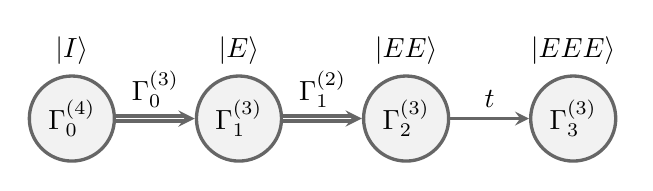
\begin{tikzpicture}[
roundnode/.style={circle, draw=black!60, fill=black!5, very thick, minimum size=0.25}
]
    %Nodes
    \node[roundnode, label={$\ket{I}$}]    
        (m0)                    {$\Gamma_0^{(4)}$};
    \node[roundnode, label={$\ket{E}$}]    
        (m1)    [right=of m0]   {$\Gamma_1^{(3)}$};
    \node[roundnode, label={$\ket{EE}$}]    
        (m2)    [right=of m1]   {$\Gamma_2^{(3)}$};
    \node[roundnode, label={$\ket{EEE}$}]    
        (m3)    [right=of m2]   {$\Gamma_3^{(3)}$};
    
    %Lines
    \draw[->, >=stealth, draw=black!60, very thick, double] 
        (m0.east) -- node[above] {$\Gamma_0^{(3)}$} (m1.west);
    \draw[->, >=stealth, draw=black!60, very thick, double]
        (m1.east) -- node[above] {$\Gamma_1^{(2)}$} (m2.west);
    \draw[->, >=stealth, draw=black!60, very thick] 
        (m2.east) -- node[above] {$t$} (m3.west);
\end{tikzpicture}
    \caption{Diagram representing the coefficient $G_{EE,EEE}$. Each node represents a state of the system (labeled above). Single line describes part of the path of the hole that is distinct in states $\ket{EE}$ and $\ket{EEE}$. Double line corresponds to common part of the walk. From the above graph one can easily read out the formula for $G_{EE,EEE}$ in terms of $\Gamma_k^{(s)}$ and $t$.}
    \label{fig:diag_EE-EEE}
\end{figure}

The mentioned diagrams consist of set nodes (circles) connected with edges (lines). Each node represents a state of the system (labeled above it). Each line ends with an arrow denoting direction of the move of the hole. Each node is associated with its weight $\Gamma_k^{(s_k)}$, where $s_k$ is equal to the number of possible states reachable from the corresponding state of $k$-th node minus the number of arrows directed at the $k$-th node. On the Bathe lattice with $z=4$ there are always 4 states reachable from each state. Thus the first node have $s_0=4$ and every other node have $s_{k>0}=3$. These numbers will be different for the self-avoiding walks on the square lattice, but general rule is the same. Single line describes part of the path of the hole that is distinct in two final states for which we calculate the coefficient of the Greens function. Each such line introduce a factor of $t$ to the coefficient. Double line represents common part of the path of the hole in both states. We denote each such line with weight of the node at which the line starts. The factor $s'_k$ for double line is equal to the number of states reachable form the node at which the line starts minus total number of lines connected to this node (double line counts as 1). This means $s'_k = s_k - 1$. As the last rule, we state that if two consecutive moves are inverse of one another (i.e. $N$ and $S$ or $E$ and $W$) they do not generate any node nor line in the graph as those moves can be reduced to identity $I$.

This summarizes creation of the graph for any coefficient we want. Now let see how we can read out the coefficient of the Greens function from such graph. First of all, this coefficient will be expressed as a fraction. Its denominator is simple, it is just a product of the self-energies of all the nodes in the graph. We split the numerator into the product of two parts. One of them corresponds to all the single lines in the graph and introduces a factor of $t$ for each such line. The other one is more complex. It will be expressed as a product of finite continued fractions,
\begin{equation}
    \prod_{k=0}^{l-1} \left(
        \Gamma_{k}^{(s'_k)}(\omega) - \K_{n=k+1}^{l-1} \frac{t^2}{\Gamma_{n}^{(s'_n)}(\omega)}
    \right),
\end{equation}
where $l$ denotes length of the common part of the moves of the hole in right and left state. This is already enough to express absolute value of the desired quantity. We need to incorporate a proper sign in the end. Again, the rule is simple, given lengths of both walks, $r$ for the right state and $c$ for the left one we have to multiply our result by $(-1)^{r+c}$. Thus in the end we can write,
\begin{equation}
\begin{split}
    \bra{\xi'_1 \xi'_2 \hdots \xi'_c}
    &\hat{G}(\omega)
    \ket{\xi_1 \xi_2 \hdots \xi_r} = \\
    &(-1)^{r+c}\frac{
    t^{r + c - 2l}
    \prod_{k=0}^{l-1} \left(
        \Gamma_{k}^{(s'_k)}(\omega) - \K_{n=k+1}^{l-1} \frac{t^2}{\Gamma_{n}^{(s'_n)}(\omega)}
    \right)
    }{
    \left(
        \prod_{k=0}^{l} \Gamma_k^{(s_k)}
    \right)
    \left(
        \prod_{k=l+1}^{r} \Gamma_k^{(s_k)}
    \right)
    \left(
        \prod_{k=l+1}^{c} \Gamma_k^{(s_k)}
    \right)
    },    
\end{split}
\end{equation}
where $\xi'_i = \xi_i$ for $i = 1,2,\hdots,l$ and  $\xi'_{l+1} \neq \xi_{l+1}$. The general formula looks complicated, but reading it from the diagram in a particular case is rather straightforward.

As a double check, let see how these diagrams work for simplest cases, which we already calculated before. We start with $G_{I,I}$. Its graph is presented below. \\
\begin{center}
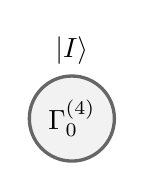
\begin{tikzpicture}[
roundnode/.style={circle, draw=black!60, fill=black!5, very thick, minimum size=0.25}
]
    %Nodes
    \node[roundnode, label={$\ket{I}$}]    
        (m0)                    {$\Gamma_0^{(4)}$};
        
\end{tikzpicture}  
\end{center}
So we immediately read out,
\begin{equation}
    G_{I,I}(\omega) = \frac{1}{\Gamma_0^{(4)}(\omega)} = \frac{1}{G_0^{-1}(\omega) - 4\Sigma_0(\omega)},
\end{equation}
which is the correct expression. Now let us work out $G_{E,E}$, \\
\begin{center}
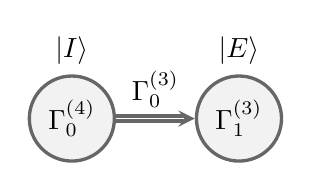
\begin{tikzpicture}[
roundnode/.style={circle, draw=black!60, fill=black!5, very thick, minimum size=0.25}
]
    %Nodes
    \node[roundnode, label={$\ket{I}$}]    
        (m0)                    {$\Gamma_0^{(4)}$};
    \node[roundnode, label={$\ket{E}$}]    
        (m1)    [right=of m0]   {$\Gamma_1^{(3)}$};
    
    %Lines
    \draw[->, >=stealth, draw=black!60, very thick, double] 
        (m0.east) -- node[above] {$\Gamma_0^{(3)}$} (m1.west);
\end{tikzpicture}
\end{center}
So we read out,
\begin{equation}
    G_{E,E}(\omega) = \frac{\Gamma_0^{(3)}(\omega)}
    {\Gamma_0^{(4)}(\omega)\Gamma_1^{(3)}(\omega)}
    = \frac{\Gamma_0^{(4)}(\omega) + \Sigma_0(\omega)}
    {\Gamma_0^{(4)}(\omega)t^2\Sigma_0(\omega)^{-1}}
    = \frac{1}{t^2}\left(
    \Sigma_0(\omega) + \Sigma_0(\omega)G(\omega)\Sigma_0(\omega)
    \right),
\end{equation}
which again is the correct expression. In the end let see $G_{N,E}$.
\begin{center}
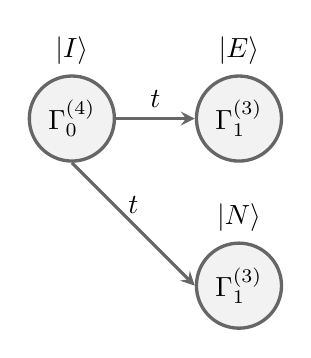
\begin{tikzpicture}[
roundnode/.style={circle, draw=black!60, fill=black!5, very thick, minimum size=0.25}
]
    %Nodes
    \node[roundnode, label={$\ket{I}$}]    
        (m0)                    {$\Gamma_0^{(4)}$};
    \node[roundnode, label={$\ket{E}$}]    
        (mE)    [right=of m0]   {$\Gamma_1^{(3)}$};
    \node[roundnode, label={$\ket{N}$}]    
        (mN)    [below=of mE]   {$\Gamma_1^{(3)}$};
    
    %Lines
    \draw[->, >=stealth, draw=black!60, very thick] 
        (m0.east) -- node[above] {$t$} (mE.west);
    \draw[->, >=stealth, draw=black!60, very thick] 
        (m0.south) -- node[above] {$t$} (mN.west);
\end{tikzpicture}
\end{center}
So we have,
\begin{equation}
    G_{N,E}(\omega) = \frac{t^2}
    {\Gamma_0^{(4)}(\omega)\left(\Gamma_1^{(3)}(\omega)\right)^2}
    = \frac{1}{t^2}\Sigma_0(\omega)G(\omega)\Sigma_0(\omega),
\end{equation}
which indeed is correct.

\subsection{Greens function with 2 rotations}
Equipped with such powerful diagrammatic notation we can now easily workout Greens function with two rotations. We are interested in the following quantity,
\begin{equation}
    G^{\text{rot}}_{m_1, m_2}(\omega) = 
    \bra{0_\sigma}R^{\dag}_{\sigma,m_1,m_2}(0) 
        \hat{G}(\omega)
    R_{\sigma,m_1,m_2}(0) \ket{0_\sigma}.
\end{equation}
Expressing $R_{\sigma,m_1,m_2}(0) \ket{0_\sigma}$ in moves notation, we can write our rotational Greens function in the following way,
\begin{equation}
    G^{\text{rot}}_{m_1,m_2}(\omega) = 
    \frac{1}{16}\sum_{\substack{
        \xi_1, \xi_2 \in D \\ 
        \xi'_1, \xi'_2 \in D
    }}
        e^{i m_1 (\varphi_{\xi_1} - \varphi_{\xi'_1})}
        e^{i m_2 (\varphi_{\xi_2} - \varphi_{\xi'_2})}
        \bra{\xi'_1 \xi'_2}\hat{G}(\omega)\ket{\xi_1 \xi_2}.
\end{equation}
So we need to calculate $\bra{\xi'_1 \xi'_2}\hat{G}(\omega)\ket{\xi_1 \xi_2}$ but fortunately not all 256 of them due to the symmetries of the system. Let us start with finding the minimal set of coefficients that have to be calculated. Formally we can introduce an equivalence relation $\equiv$, such that $G_{\eta,\eta'} \equiv G_{\mu,\mu'}$ if and only if $G_{\eta,\eta'}$ and $G_{\mu,\mu'}$ have the same graph and corresponding indices consists of the same number of moves. Relation $\equiv$ splits our set of the coefficients into equivalence classes. For each such class it is enough to know its size and to calculate its single representative. Let us therefore find all the classes with their sizes and Greens functions.
\begin{enumerate}
    \item  $[G_{NS,NS}] = \{G_{xx^{-1},yy^{-1}} : x, y \in D\}$
    \\\\$\abs{[G_{NS,NS}]} = 16$
    \begin{center}
    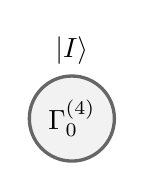
\begin{tikzpicture}[
    roundnode/.style={circle, draw=black!60, fill=black!5, very thick, minimum size=0.25}
    ]
        %Nodes
        \node[roundnode, label={$\ket{I}$}]    
            (m0)                    {$\Gamma_0^{(4)}$};
            
    \end{tikzpicture}
    \end{center}
    \begin{equation}
        G_{NS,NS}(\omega) = G_{I,I}(\omega)= \frac{1}{\Gamma_0^{(4)}(\omega)}
    \end{equation}
    
    \item  $[G_{NS,EE}] = \{G_{xx^{-1},yz}, G_{yz, xx^{-1}} : x, y, z \in D \land y \neq z^{-1}\}$
    \\\\$\abs{[G_{NS,EE}]} = 96$
    \begin{center}
    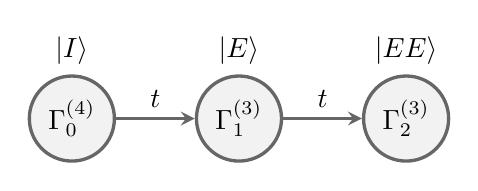
\begin{tikzpicture}[
    roundnode/.style={circle, draw=black!60, fill=black!5, very thick, minimum size=0.25}
    ]
        %Nodes
        \node[roundnode, label={$\ket{I}$}]    
            (m0)                    {$\Gamma_0^{(4)}$};
        \node[roundnode, label={$\ket{E}$}]    
            (mE)    [right=of m0]   {$\Gamma_1^{(3)}$};
        \node[roundnode, label={$\ket{EE}$}]    
            (mEE)   [right=of mE]   {$\Gamma_2^{(3)}$};
        
        %Lines
        \draw[->, >=stealth, draw=black!60, very thick,] 
            (m0.east) -- node[above] {$t$} (mE.west);
        \draw[->, >=stealth, draw=black!60, very thick] 
            (mE.east) -- node[above] {$t$} (mEE.west);
    \end{tikzpicture}
    \end{center}
    \begin{equation}
        G_{NS,EE}(\omega) = G_{I,EE}(\omega) = \frac{t^2}
        {
            \Gamma_0^{(4)}(\omega)
            \Gamma_1^{(3)}(\omega)
            \Gamma_2^{(3)}(\omega)
        }
    \end{equation}
    
    \item  $[G_{EE,EE}] = \{G_{xy,xy} : x, y \in D \land y \neq x^{-1}\}$
    \\\\$\abs{[G_{EE,EE}]} = 12$
    \begin{center}
    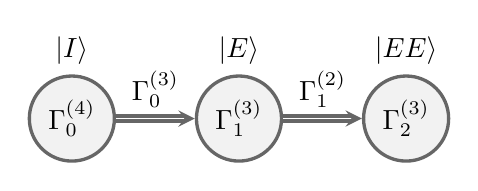
\begin{tikzpicture}[
    roundnode/.style={circle, draw=black!60, fill=black!5, very thick, minimum size=0.25}
    ]
        %Nodes
        \node[roundnode, label={$\ket{I}$}]    
            (m0)                    {$\Gamma_0^{(4)}$};
        \node[roundnode, label={$\ket{E}$}]    
            (mE)    [right=of m0]   {$\Gamma_1^{(3)}$};
        \node[roundnode, label={$\ket{EE}$}]    
            (mEE)    [right=of mE]   {$\Gamma_2^{(3)}$};
        
        %Lines
        \draw[->, >=stealth, draw=black!60, very thick, double] 
            (m0.east) -- node[above] {$\Gamma_0^{(3)}$} (mE.west);
        \draw[->, >=stealth, draw=black!60, very thick, double] 
            (mE.east) -- node[above] {$\Gamma_1^{(2)}$} (mEE.west);
    \end{tikzpicture}
    \end{center}
    \begin{equation}
        G_{EE,EE}(\omega) = \frac{
        \left(
        \Gamma_0^{(3)}(\omega)-\frac{t^2}{\Gamma_1^{(2)}(\omega)}
        \right)
        \Gamma_1^{(2)}(\omega)
        }
        {
            \Gamma_0^{(4)}(\omega)
            \Gamma_1^{(3)}(\omega)
            \Gamma_2^{(3)}(\omega)
        }
    \end{equation}
    
    \item  $[G_{EE,EN}] = \{G_{xy,xz} : x, y, z \in D \land y, z \neq x^{-1} \land y \neq z \}$
    \\\\$\abs{[G_{EE,EN}]} = 24$
    \begin{center}
    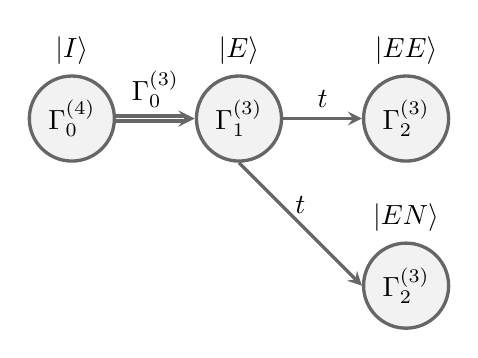
\begin{tikzpicture}[
    roundnode/.style={circle, draw=black!60, fill=black!5, very thick, minimum size=0.25}
    ]
        %Nodes
        \node[roundnode, label={$\ket{I}$}]    
            (m0)                    {$\Gamma_0^{(4)}$};
        \node[roundnode, label={$\ket{E}$}]    
            (mE)    [right=of m0]   {$\Gamma_1^{(3)}$};
        \node[roundnode, label={$\ket{EE}$}]    
            (mEE)    [right=of mE]   {$\Gamma_2^{(3)}$};
        \node[roundnode, label={$\ket{EN}$}]    
            (mEN)    [below=of mEE]   {$\Gamma_2^{(3)}$};
        
        %Lines
        \draw[->, >=stealth, draw=black!60, very thick, double] 
            (m0.east) -- node[above] {$\Gamma_0^{(3)}$} (mE.west);
        \draw[->, >=stealth, draw=black!60, very thick] 
            (mE.east) -- node[above] {$t$} (mEE.west);
        \draw[->, >=stealth, draw=black!60, very thick] 
            (mE.south) -- node[above] {$t$} (mEN.west);
    \end{tikzpicture}
    \end{center}
    \begin{equation}
        G_{EE,EN}(\omega) = \frac{
        t^2\Gamma_0^{(3)}(\omega)
        }
        {
            \Gamma_0^{(4)}(\omega)
            \Gamma_1^{(3)}(\omega)
            \left(\Gamma_2^{(3)}(\omega)\right)^2
        }
    \end{equation}
    
    \item  $[G_{EE,NE}] = \{G_{vx,yz} : v, x, y, z \in D \land v \neq y \land x \neq v^{-1} \land z \neq y^{-1}\}$
    \\\\$\abs{[G_{EE,NE}]} = 108$
    \begin{center}
    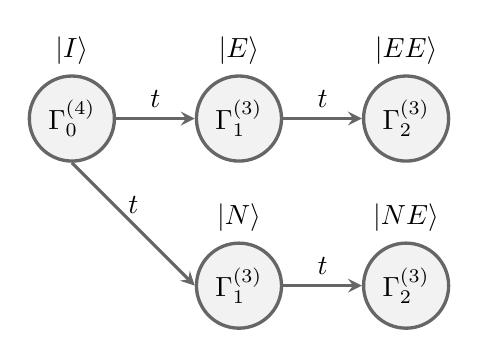
\begin{tikzpicture}[
    roundnode/.style={circle, draw=black!60, fill=black!5, very thick, minimum size=0.25}
    ]
        %Nodes
        \node[roundnode, label={$\ket{I}$}]    
            (m0)                    {$\Gamma_0^{(4)}$};
        \node[roundnode, label={$\ket{E}$}]    
            (mE)    [right=of m0]   {$\Gamma_1^{(3)}$};
        \node[roundnode, label={$\ket{EE}$}]    
            (mEE)    [right=of mE]   {$\Gamma_2^{(3)}$};
        \node[roundnode, label={$\ket{N}$}]    
            (mN)    [below=of mE]   {$\Gamma_1^{(3)}$};
        \node[roundnode, label={$\ket{NE}$}]    
            (mNE)    [below=of mEE]   {$\Gamma_2^{(3)}$};
        
        %Lines
        \draw[->, >=stealth, draw=black!60, very thick] 
            (m0.east) -- node[above] {$t$} (mE.west);
        \draw[->, >=stealth, draw=black!60, very thick] 
            (mE.east) -- node[above] {$t$} (mEE.west);
        \draw[->, >=stealth, draw=black!60, very thick] 
            (m0.south) -- node[above] {$t$} (mN.west);
        \draw[->, >=stealth, draw=black!60, very thick] 
            (mN.east) -- node[above] {$t$} (mNE.west);
    \end{tikzpicture}
    \end{center}
    \begin{equation}
        G_{EE,NE}(\omega) = \frac{
        t^4
        }
        {
            \Gamma_0^{(4)}(\omega)
            \left(\Gamma_1^{(3)}(\omega)\right)^2
            \left(\Gamma_2^{(3)}(\omega)\right)^2
        }
    \end{equation}
\end{enumerate}
We can see that if we sum all the sizes of the above equivalence classes we indeed obtain 256 total elements. We can also see it is enough to calculate 5 coefficients to fully describe all of them.

In the end, we have to incorporate the proper phase factors in front of each one of 256 terms. Since the Greens functions can only have one of 5 possible values, all we want to know is the total sum of factors in front of each one value.
\begin{enumerate}
    \item  $[G_{NS,NS}] = \{G_{xx^{-1},yy^{-1}} : x, y \in D\}$
    \\\\$\abs{[G_{NS,NS}]} = 16$
    \begin{equation}
    \frac{1}{16}\sum_{x, y \in D}
        e^{i m_1 (\varphi_{y} - \varphi_{x})}
        e^{i m_2 (\varphi_{y^{-1}} - \varphi_{x^{-1}})}
    = \frac{1}{4}\sum_{x \in D} e^{i (m_1 - m_2) \varphi_x}
    = \delta_{m_1 - m_2}
    \end{equation}
    
    \item  $[G_{NS,EE}] = \{G_{xx^{-1},yz}, G_{yz, xx^{-1}} : x, y, z \in D \land y \neq z^{-1}\}$
    \\\\$\abs{[G_{NS,EE}]} = 96$
    \begin{equation}
    \begin{split}
    &\frac{1}{16}\left(
    \sum_{\substack{
        x, y, z \in D \\ 
        y \neq z^{-1}
    }}
        e^{i m_1 (\varphi_{y} - \varphi_{x})}
        e^{i m_2 (\varphi_{z} - \varphi_{x^{-1}})}
    +
    \sum_{\substack{
        x, y, z \in D \\ 
        y \neq z^{-1}
    }}
        e^{i m_1 (\varphi_{x} - \varphi_{y})}
        e^{i m_2 (\varphi_{x^{-1}} - \varphi_{z})}
    \right) \\
    &=
    \frac{1}{16}\left(
    \sum_{\substack{
        x, y, z \in D \\ 
        y \neq z^{-1}
    }}
        e^{i m_1 (\varphi_{y} - \varphi_{x})}
        e^{i m_2 (\varphi_{z} + \varphi_{x})}
    +
    \sum_{\substack{
        x, y, z \in D \\ 
        y \neq z^{-1}
    }}
        e^{-i m_1 (\varphi_{y} - \varphi_{x})}
        e^{-i m_2 (\varphi_{z} + \varphi_{x})}
    \right) \\
    &=
    \frac{1}{4}\delta_{m_1 - m_2}
    \sum_{\substack{
        y, z \in D \\ 
        y \neq z^{-1}
    }} \left(
        e^{i (m_1 \varphi_{y} + m_2 \varphi_{z})} +
        e^{- i (m_1 \varphi_{y} + m_2 \varphi_{z})}
    \right) \\
    &=
    2\delta_{m_1 - m_2}\delta_{m_1 + m_2}\left(
        1 + e^{i m_2 \frac{\pi}{2}} + e^{-i m_2 \frac{\pi}{2}}
    \right) = 6 \delta_{m_1} \delta_{m_2}
    \end{split}
    \end{equation}
    
    \item  $[G_{EE,EE}] = \{G_{xy,xy} : x, y \in D \land y \neq x^{-1}\}$
    \\\\$\abs{[G_{EE,EE}]} = 12$
    \begin{equation}
    \frac{1}{16}
    \sum_{\substack{
        x, y \in D \\ 
        y \neq x^{-1}
    }}
        e^{i m_1 (\varphi_{x} - \varphi_{x})}
        e^{i m_2 (\varphi_{y} - \varphi_{y})}
    = \frac{3}{4}
    \end{equation}
    
    \item  $[G_{EE,EN}] = \{G_{xy,xz} : x, y, z \in D \land y, z \neq x^{-1} \land y \neq z \}$
    \\\\$\abs{[G_{EE,EN}]} = 24$
    \begin{equation}
    \begin{split}
    &\frac{1}{16}
    \sum_{\substack{
        x, y, z \in D \\ 
        y, z \neq x^{-1} \\
        y \neq z
    }}
        e^{i m_1 (\varphi_{x} - \varphi_{x})}
        e^{i m_2 (\varphi_{z} - \varphi_{y})}
    =
    \frac{1}{16}
    \sum_{\substack{
        x, y, z \in D \\ 
        y \neq z \\
        x \neq y^{-1} \\
        x \neq z^{-1} 
    }}
        e^{i m_2 (\varphi_{z} - \varphi_{y})} \\
    &=
    \frac{1}{8}
    \sum_{\substack{
        y, z \in D \\ 
        y \neq z
    }}
        e^{i m_2 (\varphi_{z} - \varphi_{y})} 
    =
    \frac{1}{2}
    \left(
        e^{i m_2 \frac{\pi}{2}} +
        e^{i m_2 \pi} +
        e^{-i m_2 \frac{\pi}{2}}
    \right) = 2\delta_{m_2} - \frac{1}{2}
    \end{split}
    \end{equation}
    
    \item  $[G_{EE,NE}] = \{G_{vx,yz} : v, x, y, z \in D \land v \neq y \land x \neq v^{-1} \land z \neq y^{-1}\}$
    \\\\$\abs{[G_{EE,NE}]} = 108$
    \begin{equation}
    \begin{split}
    &\frac{1}{16}
    \sum_{\substack{
        v, x, y, z \in D \\
        v \neq y \\
        x \neq v^{-1} \\
        z \neq y^{-1}
    }}
        e^{i m_1 (\varphi_{y} - \varphi_{v})}
        e^{i m_2 (\varphi_{z} - \varphi_{x})}
   \\ &=
    \frac{1}{16}
    \sum_{\substack{
        v, y \in D \\
        v \neq y
    }}
        e^{i (m_1 + m_2) (\varphi_{y} - \varphi_{v})}
        \left( 1 + e^{i m_2 \frac{\pi}{2}} +
        e^{-i m_2 \frac{\pi}{2}} \right)^2
   \\ &=
    \frac{1}{16}
    \sum_{\substack{
        y \in D \\
    }}
        (4\delta_{m_1 + m_2} - 1)
        (4\delta_{m_2} - e^{i m_2 \pi})^2
   \\ &=
    \frac{
        (4\delta_{m_1 + m_2} - 1)
        (4\delta_{m_2} - 1)^2    
    }{4}
    \end{split}
    \end{equation}
\end{enumerate}
Now, when we have all the phase factors, we can write our Greens function. It reads,
\begin{equation}
\begin{split}
    G^{\text{rot}}_{m_1,m_2}(\omega) &= 
    \frac{\delta_{m_1 - m_2}}{\Gamma_0^{(4)}(\omega)} +
    \frac{6 \delta_{m_1} \delta_{m_2} t^2}
        {
            \Gamma_0^{(4)}(\omega)
            \Gamma_1^{(3)}(\omega)
            \Gamma_2^{(3)}(\omega)
        } \\
    &+ \frac{3}{4} \frac{
        \left(
        \Gamma_0^{(3)}(\omega)-\frac{t^2}{\Gamma_1^{(2)}(\omega)}
        \right)
        \Gamma_1^{(2)}(\omega)
        }
        {
            \Gamma_0^{(4)}(\omega)
            \Gamma_1^{(3)}(\omega)
            \Gamma_2^{(3)}(\omega)
        } +
    \frac{
        \left(2\delta_{m_2} - \frac{1}{2}\right)
        t^2\Gamma_0^{(3)}(\omega)
        }
        {
            \Gamma_0^{(4)}(\omega)
            \Gamma_1^{(3)}(\omega)
            \left(\Gamma_2^{(3)}(\omega)\right)^2
        } \\
    &+  \frac{
            (4\delta_{m_1 + m_2} - 1)
            (4\delta_{m_2} - 1)^2    
        }{4}
        \frac{
        t^4
        }
        {
            \Gamma_0^{(4)}(\omega)
            \left(\Gamma_1^{(3)}(\omega)\right)^2
            \left(\Gamma_2^{(3)}(\omega)\right)^2
        }.
\end{split}
\end{equation}
We can see it is enough to calculate $\Gamma_0^{(4)}$, $\Gamma_0^{(3)}$, $\Gamma_1^{(3)}$, $\Gamma_1^{(2)}$ and $\Gamma_2^{(3)}$. Having $G(\omega) = G_{I,I}(\omega)$ calculated numerically for certain values of $\omega$, all we have to do is to use definition of $\Gamma_k^{(s_k)}$ and recursive relations between $\Sigma_n$ and $\Sigma_{n+1}$ to find numerical values of $G^{\text{rot}}_{m_1,m_2}(\omega)$.

Higher rotational Greens functions can be found in completely analogues way. This summarizes the case of the Bethe lattice. Let us now generalize this approach to self-avoiding walks on the 2D square lattice.

\section{Self-avoiding Walks on the 2D Square Lattice}
For the Bethe lattice we were able to arrive at powerful diagrammatic approach allowing us to easily deal with rotational Greens function despite large number of terms and quite complex overall structure of the Greens function itself. We will be able to greatly benefit form the same approach also in the case of the self-avoiding walks on the 2D square lattice. 

\subsection{Generalization from the Bethe to the 2D square lattice}
In fact the general approach that we employed before will stay untouched. There are only two generalizations that we need to introduce. The first one comes form the fact that now the potential energy of each state will depend on the path of the hole. In contrast, on the Bethe lattice only distance from the origin matters. Thus we could numerate $\Gamma_k^{(s)}$ functions with natural indices $k$. Now we will have to write $\Gamma_{\eta}^{\Delta}$ where $\eta = \xi_1 \xi_2 \xi_3 \hdots$, with each $\xi_i \in D$. 

The second generalization comes from the fact that on the square lattice the number of possible moves of the hole from certain state will depend on the path of the hole. So we can have $\Delta \subset D$. In contrast, for the Bethe lattice from each state we always had at least $z-1$ states reachable without returning.

\subsection{Local Greens function of the single hole}
The stated generalizations also have to be included in the recursive equations for the self-energy functions. Let us introduce functional $\mathcal{S}$ that takes a self-avoiding path $\xi_1 \xi_2 \hdots \xi_n$ of the hole and returns set of moves $\Delta$ that lead to self-avoiding paths $\xi_1 \xi_2 \hdots \xi_{n} \xi_{n+1}$ reachable from the path $\xi_1 \xi_2 \hdots \xi_n$. Then we can write,
\begin{equation}
    G(\omega)^{-1} = G_{I,I}(\omega) = G_I(\omega)^{-1} - \sum_{\xi_1 \in D}\Sigma_{\xi_1}(\omega), 
\end{equation}
\begin{equation}
    t^2\Sigma_{\eta}(\omega)^{-1} = G_{\eta}(\omega)^{-1} - \sum_{\xi \in \mathcal{S}(\eta)}\Sigma_{\eta\xi}(\omega),
\end{equation}
where $\eta = \xi_1 \xi_2 \hdots \xi_{n}$ is a self-avoiding walk with $\xi_i \in D$, and
\begin{equation}
    G_{\xi_1 \xi_2 \hdots \xi_{n}}(\omega)^{-1} = 
    \bra{\xi_1 \xi_2 \hdots \xi_{n}}
    \left(
        \omega - \mathcal{H}_J + E_{\textsc{gs}}
    \right)
    \ket{\xi_1 \xi_2 \hdots \xi_{n}}.
\end{equation}
Thus, the local Greens function can be written as follows,
\begin{equation}
    G(\omega) = \frac{1}{
        G_I(\omega)^{-1} - 
        \sum_{\xi_1 \in D}\left(\frac{t^2}{
            G_{\xi_1}(\omega)^{-1} - 
            \sum_{\xi_2 \in \mathcal{S}(\xi_1)}\left(\frac{t^2}{
                G_{\xi_1\xi_2}(\omega)^{-1} - \hdots
            }\right)
        }\right)
    }.
\label{eq:SquareGF}
\end{equation}
Moreover we define,
\begin{equation}
    \Gamma_{\eta}^{\Delta}(\omega) = G_{\eta}(\omega)^{-1} - \sum_{\xi \in \Delta}\Sigma_{\eta\xi}(\omega),
\end{equation}
and,
\begin{equation}
    \det T^{(\eta)}(\omega) = 
        \Gamma_{\eta}^{\mathcal{S}(\eta)}(\omega)
        \prod_{\xi \in \mathcal{S}(\eta)}
        \det T^{(\eta\xi)}(\omega).
        \label{eq:det_recursive_gamma_square}
\end{equation}
Then the local Greens function can be also expressed through diagrams in the following way, \\
\begin{center}
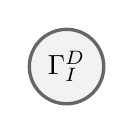
\begin{tikzpicture}[
roundnode/.style={circle, draw=black!60, fill=black!5, very thick, minimum size=0.25}
]
    %Nodes
    \node[roundnode]    
        (m0)                    {$\Gamma_I^{D}$};
        
\end{tikzpicture}  
\end{center}
\begin{equation}
    G(\omega) = \frac{1}{\Gamma_I^{D}(\omega)} = \frac{1}{G_I^{-1}(\omega) - \Sigma_E(\omega) - \Sigma_N(\omega) - \Sigma_W(\omega) - \Sigma_S(\omega)}.
\end{equation}
Note also $\Sigma_E(\omega) = \Sigma_N(\omega) = \Sigma_W(\omega) = \Sigma_S(\omega)$ as there is no process that would distinguish between 4 paths $\xi \in D$.

\subsection{Rules for the Diagrams}
New notation is slightly more complicated then the notation used for the Bethe lattice. Let us therefore restate the rules for creating the diagrams in terms of this new notation. 
\begin{enumerate}
    \item Diagram consists of nodes connected with single lines or double lines. Nodes correspond to states of the system, while lines represent the motion of the hole. Single lines represent motion distinct in the left and the right states while double lines correspond to common parts of the path.
    \item Each node is labeled with its corresponding weight $\Gamma_{\eta}^{\mathcal{S}(\eta)}$, where $\eta$ is state of the system in moves notation.
    \item Single line is denoted with $t$ as they add a factor of $t$ to the whole solution.
    \item Double line corresponding to move $\xi \in D$ and starting from the node denoted with $\Gamma_{\eta}^{\mathcal{S}(\eta)}$ is denoted with $\Gamma_{\eta}^{\mathcal{S}(\eta) \setminus \{\xi\}}$.
    \item Each line ends with arrow denoting direction of hole motion (i.e. order of moves operators $\xi \in D$) in the left and the right state.
\end{enumerate}

\subsection{Greens function with 1 rotation}
As a warm-up exercise let us work out a Greens function for a single move. Its form shall be the same as in the case of the Bethe lattice. Only notation will be different. We start with $G_{x,x} = G_{E,E}$, $x \in D$. \\
\begin{center}
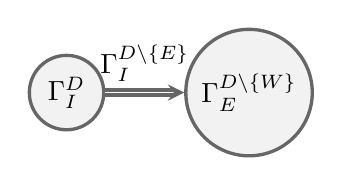
\begin{tikzpicture}[
roundnode/.style={circle, draw=black!60, fill=black!5, very thick, minimum size=0.25}
]
    %Nodes
    \node[roundnode]    
        (m0)                    {$\Gamma_I^{D}$};
    \node[roundnode]    
        (m1)    [right=of m0]   {$\Gamma_E^{D \setminus \{W\}}$};
    
    %Lines
    \draw[->, >=stealth, draw=black!60, very thick, double] 
        (m0.east) -- node[above] {$\Gamma_I^{D \setminus \{E\}}$} (m1.west);
\end{tikzpicture}
\end{center}
\begin{equation}
    G_{E,E}(\omega) = \frac{\Gamma_I^{D \setminus \{E\}}(\omega)}
    {\Gamma_I^{D}(\omega)\Gamma_E^{D \setminus \{W\}}(\omega)}.
\end{equation}
Now, let see $G_{x,y} = G_{N,E}$ where $x \neq y$.
\begin{center}
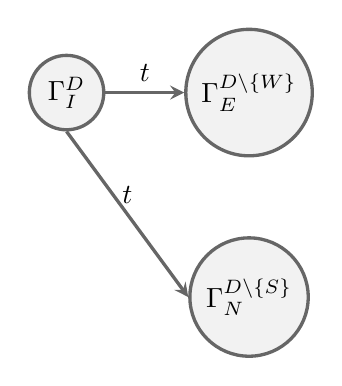
\begin{tikzpicture}[
roundnode/.style={circle, draw=black!60, fill=black!5, very thick, minimum size=0.25}
]
    %Nodes
    \node[roundnode]    
        (m0)                    {$\Gamma_I^{D}$};
    \node[roundnode]    
        (mE)    [right=of m0]   {$\Gamma_E^{D \setminus \{W\}}$};
    \node[roundnode]    
        (mN)    [below=of mE]   {$\Gamma_N^{D \setminus \{S\}}$};
    
    %Lines
    \draw[->, >=stealth, draw=black!60, very thick] 
        (m0.east) -- node[above] {$t$} (mE.west);
    \draw[->, >=stealth, draw=black!60, very thick] 
        (m0.south) -- node[above] {$t$} (mN.west);
\end{tikzpicture}
\end{center}
So we have,
\begin{equation}
    G_{N,E}(\omega) = \frac{t^2}
    {\Gamma_I^{D}(\omega)\Gamma_E^{D \setminus \{W\}}(\omega)\Gamma_N^{D \setminus \{S\}}(\omega)} = \frac{t^2}
    {\Gamma_I^{D}(\omega)\left(\Gamma_E^{D \setminus \{W\}}(\omega)\right)^2},
\end{equation}
since for $x,y \in D$ it holds that $\Gamma_x^{D \setminus \{x^{-1}\}}(\omega) = \Gamma_{y}^{D \setminus \{y^{-1}\}}(\omega)$ due to the symmetry of the system. We can see the obtained form is exactly the same as the calculated previously for the Bethe lattice,
\begin{equation}
\begin{split}
    G_m(\omega) &= 
    \frac{\Gamma_I^{D \setminus \{E\}}(\omega)}
    {\Gamma_I^{D}(\omega)\Gamma_E^{D \setminus \{W\}}(\omega)}
    +  
    \frac{\left(4\delta_m - 1\right) t^2}
    {\Gamma_I^{D}(\omega)\left(\Gamma_E^{D \setminus \{W\}}(\omega)\right)^2} \\
    &=
    \frac{1}{t^2}\Sigma_E(\omega) + \frac{4\delta_m}{t^2} \Sigma_E(\omega)G(\omega)\Sigma_E(\omega).
\end{split}
\end{equation}
where 
\begin{equation}
    \Gamma_I^{D \setminus \{E\}}(\omega) = \Gamma_I^{D}(\omega) + \Sigma_{E}(\omega) = G(\omega)^{-1} + \Sigma_{E}(\omega),
\end{equation}
and
\begin{equation}
    \Gamma_E^{D \setminus \{W\}}(\omega) = t^2 \Sigma_E(\omega)^{-1}.
\end{equation}

\subsection{Greens function with 2 rotations}
Now let investigate slightly more complicated case of the two moves. Again, we will find all the classes with their sizes and Greens functions, like we did for the Bethe lattice.
\begin{enumerate}
    \item  $[G_{EW,EW}] = \{G_{xx^{-1},yy^{-1}} : x, y \in D\}$
    \\\\$\abs{[G_{EW,EW}]} = 16$
    \begin{center}
    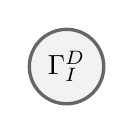
\begin{tikzpicture}[
    roundnode/.style={circle, draw=black!60, fill=black!5, very thick, minimum size=0.25}
    ]
        %Nodes
        \node[roundnode]    
            (m0)                    {$\Gamma_I^{D}$};
            
    \end{tikzpicture}
    \end{center}
    \begin{equation}
        G_{EW,EW}(\omega) = G_{I,I}(\omega)= \frac{1}{\Gamma_I^{D}(\omega)}
    \end{equation}
    
    \item  $[G_{EW,EE}] = \{G_{xx^{-1},yy}, G_{yy, xx^{-1}} : x, y \in D \}$
    \\\\$\abs{[G_{EW,EE}]} = 32$
    \begin{center}
    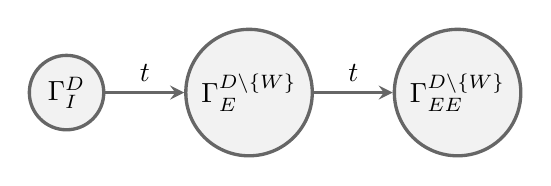
\begin{tikzpicture}[
    roundnode/.style={circle, draw=black!60, fill=black!5, very thick, minimum size=0.25}
    ]
        %Nodes
        \node[roundnode]    
            (m0)                    {$\Gamma_I^{D}$};
        \node[roundnode]    
            (mE)    [right=of m0]   {$\Gamma_E^{D \setminus \{W\}}$};
        \node[roundnode]    
            (mEE)   [right=of mE]   {$\Gamma_{EE}^{D \setminus \{W\}}$};
        
        %Lines
        \draw[->, >=stealth, draw=black!60, very thick,] 
            (m0.east) -- node[above] {$t$} (mE.west);
        \draw[->, >=stealth, draw=black!60, very thick] 
            (mE.east) -- node[above] {$t$} (mEE.west);
    \end{tikzpicture}
    \end{center}
    \begin{equation}
        G_{EW,EE}(\omega) = G_{I,EE}(\omega) = \frac{t^2}
        {
            \Gamma_I^{D}(\omega)
            \Gamma_E^{D \setminus \{W\}}(\omega)
            \Gamma_{EE}^{D \setminus \{W\}}(\omega)
        }
    \end{equation}
    
    \item  $[G_{EW,EN}] = \{G_{xx^{-1},yz}, G_{yz, xx^{-1}} : x, y, z \in D \land y \neq z \land y \neq z^{-1}\}$
    \\\\$\abs{[G_{EW,EN}]} = 64$
    \begin{center}
    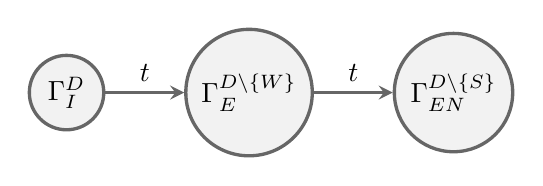
\begin{tikzpicture}[
    roundnode/.style={circle, draw=black!60, fill=black!5, very thick, minimum size=0.25}
    ]
        %Nodes
        \node[roundnode]    
            (m0)                    {$\Gamma_I^{D}$};
        \node[roundnode]    
            (mE)    [right=of m0]   {$\Gamma_E^{D \setminus \{W\}}$};
        \node[roundnode]    
            (mEN)   [right=of mE]   {$\Gamma_{EN}^{D \setminus \{S\}}$};
        
        %Lines
        \draw[->, >=stealth, draw=black!60, very thick,] 
            (m0.east) -- node[above] {$t$} (mE.west);
        \draw[->, >=stealth, draw=black!60, very thick] 
            (mE.east) -- node[above] {$t$} (mEN.west);
    \end{tikzpicture}
    \end{center}
    \begin{equation}
        G_{EW,EN}(\omega) = G_{I,EN}(\omega) = \frac{t^2}
        {
            \Gamma_I^{D}(\omega)
            \Gamma_E^{D \setminus \{W\}}(\omega)
            \Gamma_{EN}^{D \setminus \{S\}}(\omega)
        }
    \end{equation}
    
    \item  $[G_{EE,EE}] = \{G_{xx,xx} : x \in D \}$
    \\\\$\abs{[G_{EE,EE}]} = 4$
    \begin{center}
    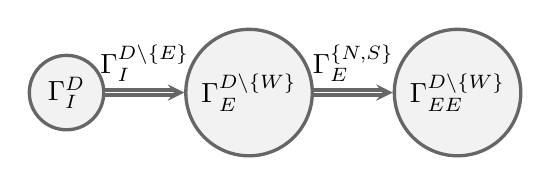
\begin{tikzpicture}[
    roundnode/.style={circle, draw=black!60, fill=black!5, very thick, minimum size=0.25}
    ]
        %Nodes
        \node[roundnode]    
            (m0)                    {$\Gamma_I^{D}$};
        \node[roundnode]    
            (mE)    [right=of m0]   {$\Gamma_E^{D \setminus \{W\}}$};
        \node[roundnode]    
            (mEE)    [right=of mE]   {$\Gamma_{EE}^{D \setminus \{W\}}$};
        
        %Lines
        \draw[->, >=stealth, draw=black!60, very thick, double] 
            (m0.east) -- node[above] {$\Gamma_I^{D \setminus \{E\}}$} (mE.west);
        \draw[->, >=stealth, draw=black!60, very thick, double] 
            (mE.east) -- node[above] {$\Gamma_E^{\{N,S\}}$} (mEE.west);
    \end{tikzpicture}
    \end{center}
    \begin{equation}
        G_{EE,EE}(\omega) = \frac{
        \left(
        \Gamma_I^{D \setminus \{E\}}(\omega)
        -\frac{t^2}{\Gamma_E^{\{N,S\}}(\omega)}
        \right)
        \Gamma_E^{\{N,S\}}(\omega)
        }
        {
            \Gamma_I^{D}(\omega)
            \Gamma_E^{D \setminus \{W\}}(\omega)
            \Gamma_{EE}^{D \setminus \{W\}}(\omega)
        }
    \end{equation}
    
    \item  $[G_{EN,EN}] = \{G_{xy,xy} : x, y \in D \land y \neq x \land y \neq x^{-1}\}$
    \\\\$\abs{[G_{EN,EN}]} = 8$
    \begin{center}
    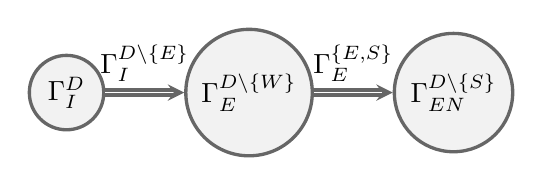
\begin{tikzpicture}[
    roundnode/.style={circle, draw=black!60, fill=black!5, very thick, minimum size=0.25}
    ]
        %Nodes
        \node[roundnode]    
            (m0)                    {$\Gamma_I^{D}$};
        \node[roundnode]    
            (mE)    [right=of m0]   {$\Gamma_E^{D \setminus \{W\}}$};
        \node[roundnode]    
            (mEN)    [right=of mE]   {$\Gamma_{EN}^{D \setminus \{S\}}$};
        
        %Lines
        \draw[->, >=stealth, draw=black!60, very thick, double] 
            (m0.east) -- node[above] {$\Gamma_I^{D \setminus \{E\}}$} (mE.west);
        \draw[->, >=stealth, draw=black!60, very thick, double] 
            (mE.east) -- node[above] {$\Gamma_E^{\{E,S\}}$} (mEN.west);
    \end{tikzpicture}
    \end{center}
    \begin{equation}
        G_{EN,EN}(\omega) = \frac{
        \left(
        \Gamma_I^{D \setminus \{E\}}(\omega)
        -\frac{t^2}{\Gamma_E^{\{E,S\}}(\omega)}
        \right)
        \Gamma_E^{\{E,S\}}(\omega)
        }
        {
            \Gamma_I^{D}(\omega)
            \Gamma_E^{D \setminus \{W\}}(\omega)
            \Gamma_{EN}^{D \setminus \{S\}}(\omega)
        }
    \end{equation}
    
    \item  $[G_{EE,EN}] = \{G_{xx,xy}, G_{xy,xx} : x, y\in D \land y \neq x \land y \neq x^{-1} \}$
    \\\\$\abs{[G_{EE,EN}]} = 16$
    \begin{center}
    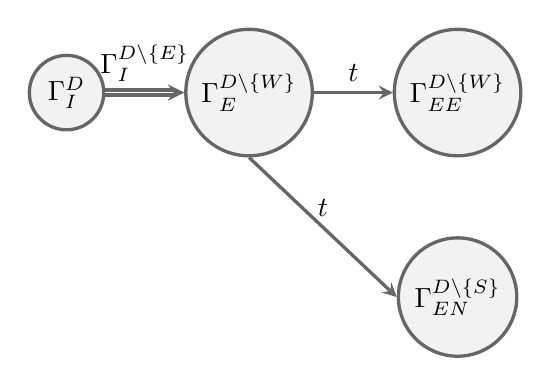
\begin{tikzpicture}[
    roundnode/.style={circle, draw=black!60, fill=black!5, very thick, minimum size=0.25}
    ]
        %Nodes
        \node[roundnode]    
            (m0)                    {$\Gamma_I^{D}$};
        \node[roundnode]    
            (mE)    [right=of m0]   {$\Gamma_E^{D \setminus \{W\}}$};
        \node[roundnode]    
            (mEE)    [right=of mE]   {$\Gamma_{EE}^{D \setminus \{W\}}$};
        \node[roundnode]    
            (mEN)    [below=of mEE]   {$\Gamma_{EN}^{D \setminus \{S\}}$};
        
        %Lines
        \draw[->, >=stealth, draw=black!60, very thick, double] 
            (m0.east) -- node[above] {$\Gamma_I^{D \setminus \{E\}}$} (mE.west);
        \draw[->, >=stealth, draw=black!60, very thick] 
            (mE.east) -- node[above] {$t$} (mEE.west);
        \draw[->, >=stealth, draw=black!60, very thick] 
            (mE.south) -- node[above] {$t$} (mEN.west);
    \end{tikzpicture}
    \end{center}
    \begin{equation}
        G_{EE,EN}(\omega) = \frac{
        t^2\Gamma_I^{D \setminus \{E\}}(\omega)
        }
        {
            \Gamma_I^{D}(\omega)
            \Gamma_E^{D \setminus \{W\}}(\omega)
            \Gamma_{EE}^{D \setminus \{W\}}(\omega)
            \Gamma_{EN}^{D \setminus \{S\}}(\omega)
        }
    \end{equation}

    \item  $[G_{ES,EN}] = \{G_{xy,xy^{-1}} : x, y \in D \land y \neq x \land y \neq x^{-1} \}$
    \\\\$\abs{[G_{ES,EN}]} = 8$
    \begin{center}
    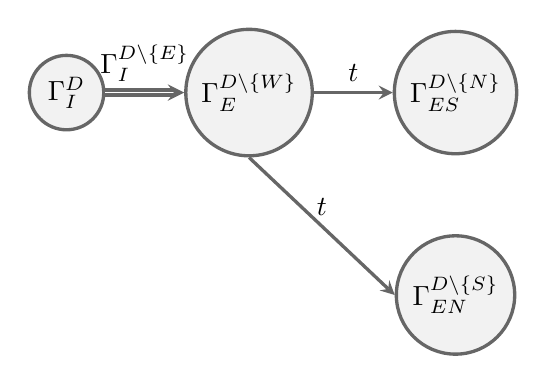
\begin{tikzpicture}[
    roundnode/.style={circle, draw=black!60, fill=black!5, very thick, minimum size=0.25}
    ]
        %Nodes
        \node[roundnode]    
            (m0)                    {$\Gamma_I^{D}$};
        \node[roundnode]    
            (mE)    [right=of m0]   {$\Gamma_E^{D \setminus \{W\}}$};
        \node[roundnode]    
            (mEE)    [right=of mE]   {$\Gamma_{ES}^{D \setminus \{N\}}$};
        \node[roundnode]    
            (mEN)    [below=of mEE]   {$\Gamma_{EN}^{D \setminus \{S\}}$};
        
        %Lines
        \draw[->, >=stealth, draw=black!60, very thick, double] 
            (m0.east) -- node[above] {$\Gamma_I^{D \setminus \{E\}}$} (mE.west);
        \draw[->, >=stealth, draw=black!60, very thick] 
            (mE.east) -- node[above] {$t$} (mEE.west);
        \draw[->, >=stealth, draw=black!60, very thick] 
            (mE.south) -- node[above] {$t$} (mEN.west);
    \end{tikzpicture}
    \end{center}
    \begin{equation}
        G_{ES,EN}(\omega) = \frac{
        t^2\Gamma_I^{D \setminus \{E\}}(\omega)
        }
        {
            \Gamma_I^{D}(\omega)
            \Gamma_E^{D \setminus \{W\}}(\omega)
            \Gamma_{ES}^{D \setminus \{N\}}(\omega)
            \Gamma_{EN}^{D \setminus \{S\}}(\omega)
        }
    \end{equation}

    \item  $[G_{EE,NN}] = \{G_{xx,yy} : x, y \in D \land x \neq y \}$
    \\\\$\abs{[G_{EE,NN}]} = 12$
    \begin{center}
    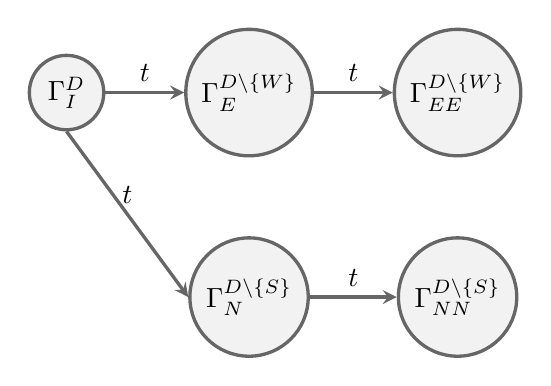
\begin{tikzpicture}[
    roundnode/.style={circle, draw=black!60, fill=black!5, very thick, minimum size=0.25}
    ]
        %Nodes
        \node[roundnode]    
            (m0)                    {$\Gamma_I^{D}$};
        \node[roundnode]    
            (mE)    [right=of m0]   {$\Gamma_E^{D \setminus \{W\}}$};
        \node[roundnode]    
            (mEE)    [right=of mE]   {$\Gamma_{EE}^{D \setminus \{W\}}$};
        \node[roundnode]    
            (mN)    [below=of mE]   {$\Gamma_N^{D \setminus \{S\}}$};
        \node[roundnode]    
            (mNE)    [below=of mEE]   {$\Gamma_{NN}^{D \setminus \{S\}}$};
        
        %Lines
        \draw[->, >=stealth, draw=black!60, very thick] 
            (m0.east) -- node[above] {$t$} (mE.west);
        \draw[->, >=stealth, draw=black!60, very thick] 
            (mE.east) -- node[above] {$t$} (mEE.west);
        \draw[->, >=stealth, draw=black!60, very thick] 
            (m0.south) -- node[above] {$t$} (mN.west);
        \draw[->, >=stealth, draw=black!60, very thick] 
            (mN.east) -- node[above] {$t$} (mNE.west);
    \end{tikzpicture}
    \end{center}
    \begin{equation}
        G_{EE,NE}(\omega) = \frac{
        t^4
        }
        {
            \Gamma_I^{D}(\omega)
            \Gamma_E^{D \setminus \{W\}}(\omega)
            \Gamma_{EE}^{D \setminus \{W\}}(\omega)
            \Gamma_N^{D \setminus \{S\}}(\omega)
            \Gamma_{NN}^{D \setminus \{S\}}(\omega)
        }
    \end{equation}
    
    \item  $[G_{EE,NE}] = \{G_{xx,yz}, G_{yz,xx} : x, y, z \in D \land x \neq y \land z \neq y \land z \neq y^{-1} \}$
    \\\\$\abs{[G_{EE,NE}]} = 48$
    \begin{center}
    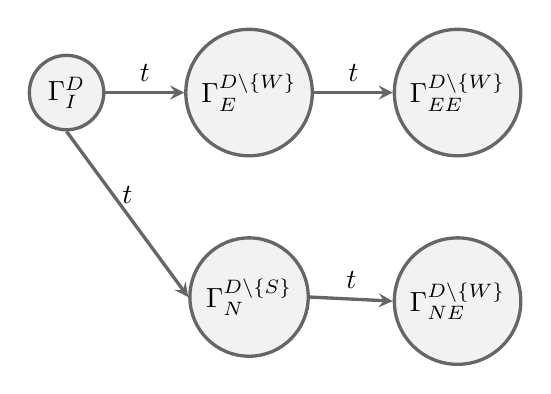
\begin{tikzpicture}[
    roundnode/.style={circle, draw=black!60, fill=black!5, very thick, minimum size=0.25}
    ]
        %Nodes
        \node[roundnode]    
            (m0)                    {$\Gamma_I^{D}$};
        \node[roundnode]    
            (mE)    [right=of m0]   {$\Gamma_E^{D \setminus \{W\}}$};
        \node[roundnode]    
            (mEE)    [right=of mE]   {$\Gamma_{EE}^{D \setminus \{W\}}$};
        \node[roundnode]    
            (mN)    [below=of mE]   {$\Gamma_N^{D \setminus \{S\}}$};
        \node[roundnode]    
            (mNE)    [below=of mEE]   {$\Gamma_{NE}^{D \setminus \{W\}}$};
        
        %Lines
        \draw[->, >=stealth, draw=black!60, very thick] 
            (m0.east) -- node[above] {$t$} (mE.west);
        \draw[->, >=stealth, draw=black!60, very thick] 
            (mE.east) -- node[above] {$t$} (mEE.west);
        \draw[->, >=stealth, draw=black!60, very thick] 
            (m0.south) -- node[above] {$t$} (mN.west);
        \draw[->, >=stealth, draw=black!60, very thick] 
            (mN.east) -- node[above] {$t$} (mNE.west);
    \end{tikzpicture}
    \end{center}
    \begin{equation}
        G_{EE,NE}(\omega) = \frac{
        t^4
        }
        {
            \Gamma_I^{D}(\omega)
            \Gamma_E^{D \setminus \{W\}}(\omega)
            \Gamma_{EE}^{D \setminus \{W\}}(\omega)
            \Gamma_N^{D \setminus \{S\}}(\omega)
            \Gamma_{NE}^{D \setminus \{W\}}(\omega)
        }
    \end{equation}
    
    \item  $[G_{EN,NE}] = \{G_{vx,yz} : v, x, y, z \in D \land x \neq v \land x \neq v^{-1} \land x,z \neq y \land z \neq y^{-1} \}$
    \\\\$\abs{[G_{EN,NE}]} = 48$
    \begin{center}
    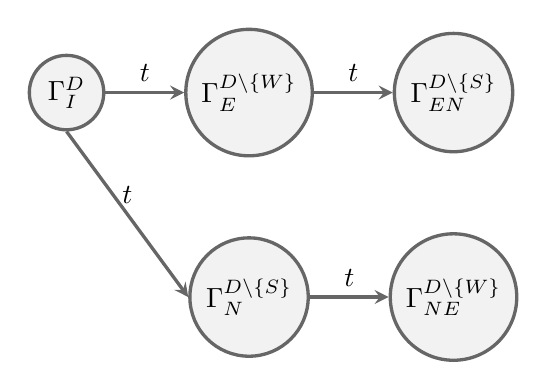
\begin{tikzpicture}[
    roundnode/.style={circle, draw=black!60, fill=black!5, very thick, minimum size=0.25}
    ]
        %Nodes
        \node[roundnode]    
            (m0)                    {$\Gamma_I^{D}$};
        \node[roundnode]    
            (mE)    [right=of m0]   {$\Gamma_E^{D \setminus \{W\}}$};
        \node[roundnode]    
            (mEE)    [right=of mE]   {$\Gamma_{EN}^{D \setminus \{S\}}$};
        \node[roundnode]    
            (mN)    [below=of mE]   {$\Gamma_N^{D \setminus \{S\}}$};
        \node[roundnode]    
            (mNE)    [below=of mEE]   {$\Gamma_{NE}^{D \setminus \{W\}}$};
        
        %Lines
        \draw[->, >=stealth, draw=black!60, very thick] 
            (m0.east) -- node[above] {$t$} (mE.west);
        \draw[->, >=stealth, draw=black!60, very thick] 
            (mE.east) -- node[above] {$t$} (mEE.west);
        \draw[->, >=stealth, draw=black!60, very thick] 
            (m0.south) -- node[above] {$t$} (mN.west);
        \draw[->, >=stealth, draw=black!60, very thick] 
            (mN.east) -- node[above] {$t$} (mNE.west);
    \end{tikzpicture}
    \end{center}
    \begin{equation}
        G_{EN,NE}(\omega) = \frac{
        t^4
        }
        {
            \Gamma_I^{D}(\omega)
            \Gamma_E^{D \setminus \{W\}}(\omega)
            \Gamma_{EN}^{D \setminus \{S\}}(\omega)
            \Gamma_N^{D \setminus \{S\}}(\omega)
            \Gamma_{NE}^{D \setminus \{W\}}(\omega)
        }
    \end{equation}
\end{enumerate}
In total 256 elements split across 10 distinct classes of coefficients. In the end, we just have to work out phase factors in front of each class. This task is trivial and can be done numerically with ease. 

\end{document}